\documentclass[preprint,12pt]{elsarticle}
\usepackage{amsmath,amssymb}
\usepackage{booktabs}
\usepackage{array}
\usepackage{calc}
\usepackage{longtable}
\usepackage{graphicx}
\usepackage{svg}
\setkeys{Gin}{width=\linewidth,keepaspectratio}
% Let Elsevier's float algorithm place figures at the top, bottom, or on a
% dedicated float page. A global [H] placement creates sparse pages and can
% separate a figure from the paragraph that introduces it.
\usepackage{float}
\usepackage[hyphens]{url}
\usepackage{microtype}
\usepackage{hyperref}
\hypersetup{colorlinks=true,urlcolor=blue,linkcolor=black,citecolor=black}
\makeatletter
\g@addto@macro\UrlBreaks{\do\-}
\makeatother
% Keep dedicated float pages top-aligned so figures do not appear vertically
% centered with an avoidable blank band above them.
\makeatletter
\setlength{\@fptop}{0pt}
\setlength{\@fpsep}{12pt}
\makeatother
\providecommand{\tightlist}{\setlength{\itemsep}{0pt}\setlength{\parskip}{0pt}}
\providecommand{\real}[1]{#1}
\sloppy
\raggedbottom
\journal{Pervasive and Mobile Computing}
\begin{document}
\begin{frontmatter}
\title{Migration-Guarded Local Reconfiguration Under Persistent Hotspots in Mobile Edge Systems}
\author[inst1,inst2]{Jeng-Shyang Pan}
\ead{jspan@ieee.org}
\author[inst1]{Peng-Yu Duan}
\ead{202483060107@sdust.edu.cn}
\author[inst1]{Li-Fa Liu}
\ead{202282060085@sdust.edu.cn}
\author[inst1]{Qing-Yong Yang}
\ead{yang_qy@sdust.edu.cn}
\author[inst3]{Shu-Chuan Chu\corref{cor1}}
\ead{100130@nuist.edu.cn}
\cortext[cor1]{Corresponding author.}
\address[inst1]{College of Computer Science and Engineering, Shandong University of Science and Technology, Qingdao 266590, China}
\address[inst2]{Department of Information Management, Chaoyang University of Technology, Taichung 41349, Taiwan}
\address[inst3]{School of Artificial Intelligence, Nanjing University of Information Science and Technology, Nanjing 210044, China}
\begin{abstract}
Persistent local hotspots can make slot-wise placement recomputation incur migration churn. We study whether retaining a repaired placement can improve service while limiting reconfiguration. BudgetedLNS is an implementation-level, state-preserving local search that ranks multi-resource pressure, bounds the candidate pool, and applies lexicographic acceptance by satisfaction, admitted-to-admitted node changes, and admitted latency. Local trials are guarded against a current-slot repaired reference, while total inter-slot node changes are audited separately; the latter can exceed the local-trial budget when the reference itself changes. Across 30 paired runs of 180 tasks over 200 slots and three persistent-hotspot profiles, the frozen 5\% setting improves satisfaction over the slot-wise MPC rollout comparator by 7.82--8.55 percentage points and reduces recorded admitted-to-admitted node changes by 96.39--96.55\%; gains over the implemented HIVE comparator are 9.65--13.82 points with 96.74--96.88\% fewer recorded node changes. Sensitivity at 1\%, 5\%, and 10\% reports inter-slot budget excesses. A true local-search-off ablation increases satisfaction by 9.30--13.60 percentage points in the three tested hotspot profiles, but also increases simulator solver time and does not uniformly reduce the migration-volume proxy. The evidence is limited to this simulator, load, and hotspot protocol; 5\% is not claimed to be universally optimal.
\end{abstract}
\begin{keyword}
mobile edge computing \sep service migration \sep local search \sep
placement \sep persistent hotspot
\end{keyword}
\end{frontmatter}
\section{Introduction}\label{introduction}

Mobile edge placement must maintain service while task mobility and
infrastructure conditions change. Mobile-edge computing and
computation-offloading surveys establish the importance of joint
communication and computation decisions
\citep{mach2017mec, mao2017survey}. A persistent local compute,
communication, or coupled resource degradation is especially difficult
because it can make a previously feasible placement unsafe for many
consecutive slots. The operational objective is not only high service
satisfaction, but also a controlled amount of placement change:
migration consumes data-transfer capacity and can itself disrupt
service.

A natural response is to solve a new placement problem at every slot.
That strategy discards the placement continuity already present in a
repaired schedule, and it can generate many more moves than the local
disturbance requires. Conversely, never changing the schedule leaves the
affected resource overloaded. The unresolved question addressed here is
narrow but practical: after a persistent local hotspot appears, how can
a controller use the existing schedule while retaining an explicit
per-slot local-search budget and exposing any inter-slot budget excess?

We answer this question with BudgetedLNS. Its central design choice is
to treat the prior repaired schedule as the starting point rather than
as disposable history. The method detects multi-resource pressure, ranks
risk-exposed tasks, restricts the candidate pool to at most three times
the move budget, and accepts a candidate only if it improves a
lexicographic objective: satisfaction first, then fewer admitted-to-admitted
node changes, then
lower admitted latency. A common post-solver safety repair enforces resource
feasibility. The operational contract is explicit: local trials that
exceed the current-reference move budget are rejected. Total inter-slot
node changes are recorded separately, including any excess above that
local-trial budget; such an excess is not itself a failed local guard.
The 5\% setting is therefore a local-trial budget guard with recorded
inter-slot budget excesses, not a universal absolute migration bound.

The paper makes three bounded contributions.

\begin{enumerate}
\def\labelenumi{\arabic{enumi}.}
\tightlist
\item
  It defines an auditable, repair-aware local reconfiguration protocol for persistent
  hotspots, explicitly separating service performance, migration cost,
  and repair feasibility.
\item
  It provides a state-preserving BudgetedLNS solver with multi-resource pressure
  localization, bounded candidate exploration, lexicographic acceptance,
  and shared feasibility repair.
\item
  It evaluates the solver in a paired, 30-run, 200-slot protocol on
  three persistent-hotspot mechanisms. The results establish a
  service--node-change advantage over the slot-wise MPC rollout and implemented HIVE
  comparator only within the stated simulator scope.
\end{enumerate}

\section{Related Work and Positioning}\label{related-work-and-positioning}

Edge and mobile-edge computing research has developed a broad
optimization space spanning system architecture, communication,
computation, and resource-allocation decisions
\citep{shi2016edge, mach2017mec, mao2017survey, abbas2018mec}. Recent
C-RAN/MEC studies also examine joint edge-service deployment and
user-satisfaction-driven offloading~\citep{pan2024joint,yang2024satisfaction}.
This
literature motivates dynamic placement, but it does not determine how
much of a feasible placement should be retained after a local persistent
disturbance.

Mobility-aware placement and migration research explicitly considers
where a service should follow a moving user. Survey and scheduling work
frames service migration as a joint latency, mobility,
container-placement, and resource-management problem
\citep{wang2018migration, oleghe2021migration}. Representative studies
investigate dynamic placement \citep{ouyang2018follow, zhao2020maesp},
proactive microservice placement and migration \citep{ray2020proactive},
probabilistic mobility-aware migration \citep{xu2021pdma}, and
digital-twin-assisted migration \citep{bozkaya2023dtmigration}. Other
systems combine caching with migration
\citep{li2021cachemigration, li2022dqnmigration} or study scalable
migration orchestration
\citep{brandherm2022bigmec,brandherm2024bigmecsoftware}. BigMEC is particularly
relevant because its public implementation exposes a scalable,
non-displacing greedy migration rule. We therefore include a code-derived,
equal-priority BigMEC greedy adapter as an external reproducible baseline;
the adapter is not presented as a reproduction of the complete BigMEC
learning system or its San Francisco topology. Our question is
narrower: given a current disturbed state and a prior repaired
placement, can the controller preserve useful placement continuity under
an explicit per-slot local-search budget?

Online MEC controllers also use stability- and learning-oriented
formulations for dynamic offloading
\citep{mao2016dynamic, bi2021lyapunov}. Online placement and offloading
have been studied with asynchronous decisions
\citep{li2021asyncoffload}, two-timescale control
\citep{li2023twotimescale}, and graph-based learning for adaptive
microservice placement
\citep{chen2024adaptiveplacement, ray2024learningmigration}. More
general online reconfiguration has also been analyzed for edge-cloud
systems \citep{hou2016reconfig}. BudgetedLNS is not presented as a
replacement for these controller families. It instead instantiates
large-neighborhood-search principles \citep{pisinger2010lns} for a
constrained reconfiguration contract: pressure-localized task selection,
a candidate pool bounded by the move budget, lexicographic acceptance,
and a common feasibility repair. The evaluation therefore compares
against slot-wise full rescheduling, the implemented HIVE comparator, and
the public-code-derived BigMEC greedy adapter, and it states no
cross-topology or deployment generalization.

\section{System Model and Objective}\label{system-model-and-objective}

At slot \(t\), each of \(N=180\) persistent tasks is either rejected or
assigned to one admissible edge resource. Let \(x_t\) denote the
placement, \(s_t(x_t)\) the simulator-defined slot satisfaction score,
and \(c_t(x_t,x_{t-1})\) the number of tasks whose assignment changes
from one nonzero edge node to a different nonzero edge node between
slots. Admission of a previously rejected task and rejection of a
previously admitted task are service-state transitions, not migrations.
The reported \texttt{MigrationMB} metric is a profile-derived volume
proxy: for each admitted-to-admitted move it sums the simulator's
scaled layer-data vector, in MB. It is not a measurement of runtime
memory residency, packet traffic, or a complete container-state transfer
trace. Resource capacities and
communication conditions vary with the scenario, while task mobility is
seeded identically across paired methods.

The simulator used five heterogeneous edge nodes. Each task belongs to
one of three DNN profiles: VGG16 (20\%, base deadline 2.0 s), ResNet50
(50\%, 1.0 s), or MobileNetV2 (30\%, 0.5 s). At a slot, task deadlines
follow \(d_i(t)=\max\{0.12,d_i(0)[0.93+0.07\sin(2\pi(t-1)/20+i/17)]\}\).
Positions are expressed in meters. In every slot, each user is sampled
around its initial position, rather than displaced from its preceding-slot
position:
\begin{equation}
 p_i(t)=\operatorname{clip}_{[0,1000]^2}
 \bigl(p_i(0)+\epsilon_{i,t}\bigr),\qquad
 \epsilon_{i,t}\sim\mathcal N(0,35^2 I_2)\ {\rm m}.
\end{equation}
The seeded displacement draws are independent across slots; this is
position jitter around a fixed anchor, not a random-walk trajectory. A slot
is a decision index, with no specified physical duration. The migration
guard is therefore a count per decision update and cannot be converted to
a migration rate or a mobility speed in meters per second. Node 1 has compute capacity 350,
bandwidth 40 Mb/s, and 8192 MB memory; nodes 2--3 have compute capacity
250, bandwidth 20 Mb/s, and 4096 MB memory; nodes 4--5 have compute
capacity 180, bandwidth 40 Mb/s, and 2048 MB memory. These values are
the fixed simulator configuration used in all formal cells.

For a placement, the load at node \(f\) is
\(r_f=\sum_i x_{if}\mathrm{Comp}_{if}/\bar d\), where \(\bar d\) is the
mean slot deadline. This execution-time load proxy feeds the queue multiplier:
\(q_f=1+r_f/[2(1-r_f+10^{-6})]\) for \(r_f<0.99\), and is set to a large
penalty otherwise. For an admitted task, latency is
\(\ell_{if}=\mathrm{Comm}_{if}+\mathrm{Comp}_{if}+\mathrm{Comp}_{if}\max(q_f-1,0)+5\times10^{-4}n_f^2\),
where \(n_f\) is the number of tasks assigned to node \(f\). A task is
satisfied only when it has exactly one assignment, its node stays below
the memory and load limits, and \(\ell_{if}\le d_i(t)\). The reported
satisfaction is \(100N^{-1}\sum_i\mathbb{1}[i\text{ is satisfied}]\).

BudgetedLNS uses a local-trial node-change guard
\(B=\max(1,\lceil\rho N\rceil)\). Its reference is
\(\bar x_t=\mathcal R_t(x_{t-1})\), the previous delivered placement
rebuilt under the current slot's inputs by the shared repair operator.
Local trials are screened using \(c_t(x,\bar x_t)\le B\), whereas the
reported inter-slot changes use \(c_t(x_t,x_{t-1})\). These references
are different when current resource, deadline, or communication inputs
cause incumbent revalidation to change the placement. The recorded excess
is
\(\max\{0,c_t(x_t,x_{t-1})-B\}\). The legacy CSV field
\texttt{RepairOverride} flags an enabled guard together with a positive
inter-slot excess; it does not establish that the terminal repair changed
an already repaired accepted trial. The first slot has no previous
placement and records zero inter-slot changes.

The frozen primary setting uses \(\rho=0.05\), hence \(B=9\).
We report mean satisfaction, total admitted-to-admitted node changes, the
profile-derived \texttt{MigrationMB} proxy, admitted and rejected task
counts, and inter-slot budget-excess events over 200 slots. Admission and
rejection transitions remain outside the node-change count. The runner
applies the same terminal repair and reporting evaluator to every method;
this is a common delivery policy, not an absolute migration guarantee.

\begin{longtable}[]{@{}
  >{\raggedright\arraybackslash}p{(\columnwidth - 2\tabcolsep) * \real{0.50}}
  >{\raggedright\arraybackslash}p{(\columnwidth - 2\tabcolsep) * \real{0.50}}@{}}
\caption{Frozen simulator and migration-guard parameters.}\\
\toprule
Parameter & Value used in the reported experiments \\
\midrule
\endhead
Edge nodes & 5 heterogeneous nodes \\
Tasks & 180 persistent tasks: 20\% VGG16, 50\% ResNet50, 30\%
MobileNetV2 \\
Base task deadlines & 2.0 s, 1.0 s, and 0.5 s for VGG16, ResNet50, and
MobileNetV2 \\
Horizon and replications & 200 slots and 30 paired seeds per scenario \\
Node 1 resources & Compute 350; bandwidth 40 Mb/s; memory 8192 MB \\
Nodes 2--3 resources & Compute 250; bandwidth 20 Mb/s; memory 4096 MB \\
Nodes 4--5 resources & Compute 180; bandwidth 40 Mb/s; memory 2048 MB \\
Mobility model & Independent Gaussian position jitter around initial
positions; standard deviation 35 m; clipped to a 1000 m by 1000 m square;
no physical slot duration \\
Persistent compute hotspot & Node 1 compute capacity at 55\% of
baseline \\
Persistent link hotspot & Node 2 bandwidth at 35\% of baseline \\
Persistent coupled hotspot & Node 1 compute at 60\%, node 2 bandwidth at
40\%, node 2 memory at 70\% \\
Primary BudgetedLNS fraction & \(\rho=0.05\), giving \(B=9\) trial-level moves; total inter-slot changes may exceed it \\
Sensitivity fractions & 0.01, 0.05, and 0.10 \\
Candidate-pool limit & At most \(3B\) risk-ranked tasks \\
Pressured nodes & Two nodes with the highest pressure score \\
HIVE controller limits & Five candidate cells, two target cells, and
four edits \\
BigMEC adapter & Equal priority; five-node neighborhood; utility
\(-\)(communication + computation latency); non-displacing greedy moves \\
MPC rollout baseline & Three-step rollout, discount 0.7, two
immediate-node candidates \\
Bootstrap and randomization & 20,000 paired bootstrap resamples; 100,000
sign flips; Holm correction \\
\bottomrule
\end{longtable}

\section{Migration-guarded BudgetedLNS}\label{budgetedlns}

\begin{figure}[!htbp]
\centering
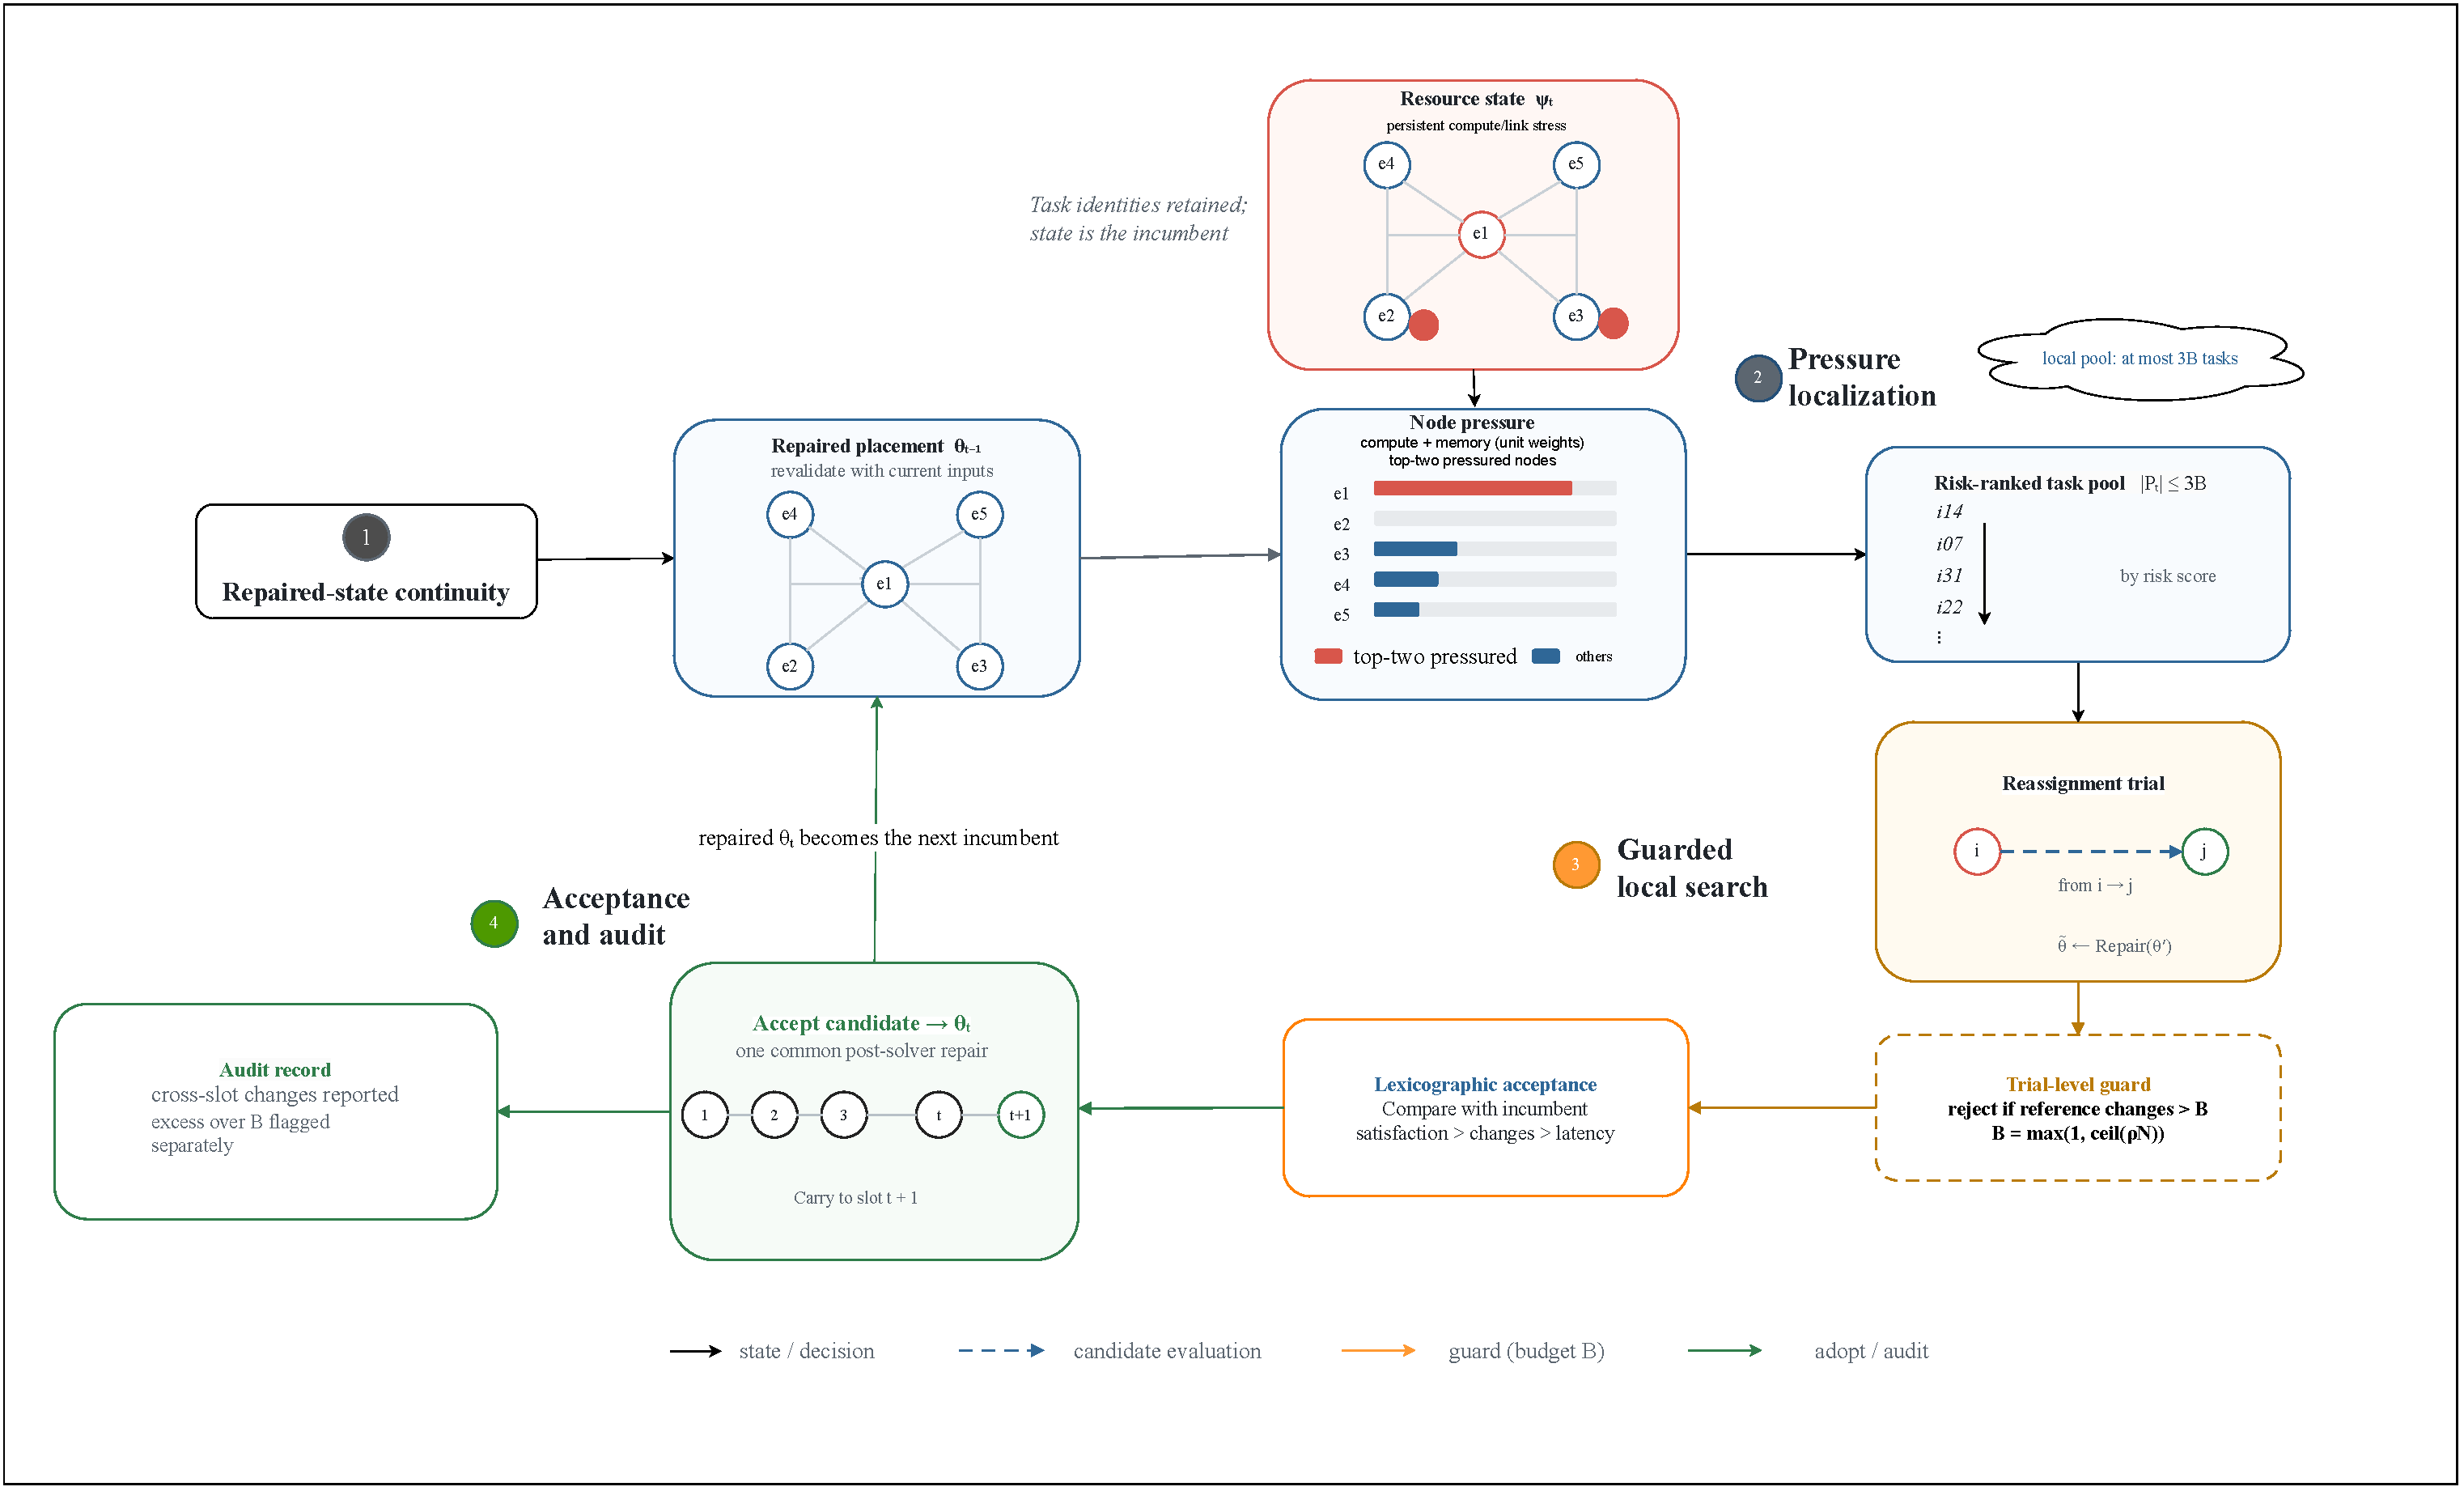
\includegraphics[width=\linewidth]{Fig1.pdf}
\caption{BudgetedLNS workflow with state carry-over and inter-slot accounting. Current-slot revalidation forms the reference for local-trial node changes. The audit instead compares delivered placements across consecutive slots; it does not attribute an excess to terminal repair. Node pressure uses computation and memory only.}
\end{figure}

\subsection{State-preserving initialization and pressure localization}\label{state-preserving-initialization-and-pressure-localization}

At slot \(t>1\), let \(\theta_{t-1}\) be the placement delivered in
the preceding slot. The solver first constructs
\(\bar\theta_t=\mathcal R_t(\theta_{t-1})\) using current-slot
inputs, and initializes the local search with \(\bar\theta_t\).
Thus, state preservation retains a revalidated incumbent rather than
assuming that the preceding placement remains feasible after the
environment changes. If no size-compatible previous placement exists,
the solver obtains an MPC rollout placement and repairs it. The two nodes
with the largest pressure scores under the initialized placement supply
the initially admitted tasks considered for local search.

\subsection{Bounded repair neighborhood}\label{bounded-repair-neighborhood}

The local-trial budget is \(B=\max(1,\lceil\rho N\rceil)\).
The risk-ranked candidate pool contains at most \(3B\) tasks from the
selected nodes. Each task initiates reassignment trials; every trial is
repaired before scoring and is rejected if its admitted-to-admitted
node-change count relative to \(\bar\theta_t\) exceeds \(B\).
This limits the initiating tasks and the admissible repaired local
proposals. The repair itself still scans the full placement and may
change admission states or assignments outside the initiating task.
Consequently, neither the pool bound nor the local guard bounds all
placement-state transitions or all repair work.

\subsection{Lexicographic acceptance and shared repair}\label{lexicographic-acceptance-and-shared-repair}

The solver compares repaired candidates by higher satisfaction, then fewer
admitted-to-admitted node changes from \(\bar\theta_t\), then lower
mean latency over admitted tasks. Satisfaction and latency comparisons use
a tolerance of \(10^{-10}\); the migration-count comparison is exact.
Exact ties retain the incumbent, and nodes are examined in ascending index
order. The search loop stops initiating further tasks once its accepted
reference-relative move count reaches \(B\), so it can stop below \(B\)
when a full-repair proposal changes multiple tasks. An accepted trial is already a
repaired placement. A final repair inside the solver and the runner's
common post-solver repair use the same current inputs; they do not add a
new search stage.

The guard controls optional local-search decisions after current-slot
revalidation. It does not constrain the changes required to form
\(\bar\theta_t\) from \(\theta_{t-1}\). Therefore, a recorded
inter-slot excess can occur even when local search leaves
\(\bar\theta_t\) unchanged. The guard's purpose is local
controllability and auditability; a small mean-satisfaction ablation effect
is not evidence of an additional performance mechanism.

\subsection{Deterministic shared feasibility repair}\label{deterministic-shared-feasibility-repair}

The common repair rebuilds a placement from an empty assignment in
ascending order of each task's minimum compute time. For the cell DNN
profiles used in these experiments, the simulated per-task memory proxy
sums the scaled layer-data entries; it is not a measured peak
runtime-memory footprint. The repair
first tries its input node (node 1 is the implementation's default when
the input row is unassigned), retaining that node when accumulated memory
fits, normalized load is below 0.95, and the newly inserted task meets its
latency allowance at that insertion step. If retention fails, it chooses
the lowest-latency node among those satisfying the memory and 0.95 load
tests. This fallback does \emph{not} require the task to meet its latency
allowance. If no resource-feasible node exists, the task is left
unassigned. For a candidate insertion on node \(f\), the context term is
\(5\times10^{-4}(n_f+1)^2\) seconds, where \(n_f\) is the number
already placed there before insertion.

Later insertions increase a node's load and task count, and can make an
earlier admitted task late. The repair does not perform a final
deadline-based deletion pass. Instead, the reporting evaluator recomputes
the completed placement's resource status and every admitted task's
latency, counting an admitted but late task as unsatisfied. Resource
feasibility and deadline satisfaction are therefore different outcomes.
For example, the compute-hotspot BudgetedLNS cell admits 139.21 tasks on
average, while 61.67\% satisfaction corresponds to about 111.01 timely,
resource-feasible tasks out of 180.

With identical current inputs, task order, and numerical tie handling,
repair is idempotent on its own outputs. This follows task by task: each
repeated pass sees the same accumulated state before the next task, and
either retains the same node or repeats the same deterministic fallback.
Changing the slot inputs invalidates this fixed-input argument. A
separate diagnostic using three scenarios, two budgets, one seed per cell,
and 60 slots per cell checked 360 slot states. Repeating repair changed
neither the repaired reference nor the repaired solver output in any
state, and all local guards held. Nevertheless, 20 inter-slot budget
exceedances occurred, including seven with an unchanged local-search
incumbent. This diagnostic verifies the distinction between revalidation,
local search, and inter-slot accounting; it is not an additional
performance comparison or a statistical estimate over the formal runs.

\subsection{Algorithmic contract}\label{algorithmic-contract}

Node pressure in the released implementation contains computation and
memory terms only:
\begin{equation}
 \pi_f(\theta)=
 \frac{\sum_i\theta_{if}\mathrm{Comp}_{if}}
 {\max(\bar d,10^{-9})}
 +\frac{\sum_i\theta_{if}m_i}{\max(C_f^{\rm mem},1)}.
\end{equation}
Here \(\bar d=\max(N^{-1}\sum_i d_i,10^{-9})\) in the solver's pressure
calculation; the repair and evaluator use their own implemented deadline
floors. The memory requirement \(m_i\) and capacity \(C_f^{\rm mem}\)
are in the simulator's MB-scaled units, and the memory denominator floor is 1 MB. Both dimensionless
terms have weight one; there is no
across-node min--max normalization. Communication is not a separate node
pressure term. It enters the task-risk score
\begin{equation}
 r_i=\frac{\mathrm{Comm}_{if}+\mathrm{Comp}_{if}}
 {\max(d_i,10^{-9})}
\end{equation}
for a task initially assigned to node \(f\). The two pressure-ranked
nodes are selected once before the local loop, and at most \(3B\)
tasks are retained in descending risk order.

\textbf{Algorithm 1. BudgetedLNS with explicit reference and accounting}

\begin{verbatim}
Input: current inputs z_t, previous delivered theta_(t-1), rho
B <- max(1, ceil(rho N))
reference <- SharedRepair(theta_(t-1); z_t)
  [if no previous placement: repair an initial MPC rollout]
theta <- reference
H <- two nodes with highest pressure under theta
P <- risk-ranked admitted tasks assigned to H; keep at most 3B
for each task i in P while moves(theta, reference) < B do
    best <- theta
    for each candidate node f do
        trial <- SharedRepair(assign i to f in theta; z_t)
        if moves(trial, reference) <= B then
            if Better(trial,best) then
                best <- trial
            end if
        end if
    end for
    theta <- best
end for
return SharedRepair(theta; z_t)
Runner: apply the same repair; report moves(theta, theta_(t-1))
Audit: excess <- max(0, reported inter-slot moves - B)
\end{verbatim}

The primary setting has \(\rho=0.05\), \(N=180\), and \(B=9\).
At most \(M\min(N,3B)\) task--node trials are initiated. A task
that remains admitted skips its current node, but a task dropped by an
earlier repair can require all \(M\) node trials; thus
\(3B(M-1)\) is not an unconditional bound. This count excludes the
initialization and repeated full-placement repair passes.
This is a bound on trial initiation only, not on total decision-layer work.
Each repair invocation first computes a memory proxy for all \(N\) tasks
and then processes the full task list, scanning up to \(M\) nodes when
retention fails; its worst-case scan cost is therefore \(O(NM)\). A
single local-search invocation can invoke repair for initialization, each
candidate trial, and final feasibility processing. The candidate-pool bound
does not cap this repair work or the cost of the simulator evaluator.

\section{Experimental Protocol}\label{experimental-protocol}

\subsection{Frozen paired evaluation}\label{frozen-paired-evaluation}

The primary experiment uses 30 independent paired runs for each of three
persistent-hotspot scenarios: compute, link, and coupled
compute/link/memory. Each run has 200 slots and \texttt{N=180} tasks.
All methods receive identical task instances, mobility perturbations,
hotspot states, final repair, metric implementation, and scenario/run
seed. The primary comparison is BudgetedLNS versus the slot-wise MPC
rollout comparator (code label \texttt{FullResched}). HIVE is
evaluated only as an internally implemented hierarchical comparator, and the
code-derived, equal-priority, non-displacing BigMEC greedy adapter is an
external reproducible baseline. All four methods use identical formal
cells. In every slot, compute hotspots reduce node 1
compute capacity to 55\% of baseline; link hotspots reduce node 2
bandwidth to 35\%; and coupled hotspots reduce node 1 compute capacity
to 60\%, node 2 bandwidth to 40\%, and node 2 memory to 70\%. The
degradation begins at the first slot and remains active throughout the
200-slot horizon.

For transparent interpretation, we pre-specify descriptive comparison
thresholds: a satisfaction difference whose 95\% confidence interval is
not below -1 percentage point, a node-change reduction of at least 30\%,
and a Holm-adjusted sign-flip \(p<0.05\) in at least two scenarios. These
thresholds are reporting conventions for this manuscript, not a validated
acceptance test or a preregistered claim. We report the number and
magnitude of inter-slot budget excesses explicitly; the 5\% setting is a
trial-level guard and is not treated as an absolute bound on the repaired
output.

\subsection{Baselines, pairing, and reporting}\label{baselines-pairing-and-reporting}

The method labelled \texttt{FullResched} in the code is a slot-wise MPC
rollout comparator, not an oracle for globally optimal re-scheduling. It
recomputes a placement independently at each slot with the implemented
MPC rollout solver. It orders tasks by deadline, examines
the two best immediate nodes, uses a three-step rollout with discount
0.7, and penalizes memory, overload, and deadline violations before the
common final repair. The HIVE comparator is the implemented hierarchical
controller: it discovers fragility cells, estimates propagation, plans
interventions, realizes sparse micro-edits, and runs a three-step
counterfactual stabilization check. Its default controller limits are
five candidate cells, two target cells, and four edits. The BigMEC adapter
maps a service to a persistent DNN task, assigns unit priority, treats the
five nodes as the destination neighborhood, and maximizes negative
communication-plus-computation latency subject to DNN-memory capacity.
It follows the public non-displacing greedy contract but then receives the
same final Safe Harbor repair as every other method. It does not execute
the original BigMEC learning components, 50-node topology, or trace.
The adapter was audited against the GPL-3.0 repository at
\url{https://github.com/flbrandh/MEC-Simulator-2-BigMEC}, commit
\texttt{a586ae3b98119f83bb7883bd94ea95b1fbed7a8c}.
Within each
scenario, a paired run uses the same task instance, mobility sequence,
persistent degradation trace, final repair, and metric implementation
for every method. The reported paired confidence intervals and
Holm-adjusted sign-flip tests therefore evaluate within-seed method
differences. This evaluation does not claim a comparison with every
controller class, a real deployment, or generalization across topology
and load.

\subsection{Hotspot onset and component ablation}\label{hotspot-onset-and-component-ablation}

The hotspot-onset experiment first runs 50 normal slots to form a feasible,
method-specific deployment. At slot 51, the designated compute, link, or
coupled degradation is applied and remains active through slot 200. We
report trajectories and post-onset outcomes so that adaptation is not
confounded with first-slot initialization.

The component experiment uses the same slot-51 onset protocol and
compares operational variants of the frozen 5\% method. The first
variant replaces state-preserving initialization with a fresh MPC rollout
at every slot. The second replaces the pressure-localized, at-most-\(3B\)
pool with all currently admitted tasks. The third disables the 5\% local
trial guard while retaining state preservation and pressure localization.
All variants retain the common feasibility repair, inputs, seeds, and
metrics. The global-pool variant jointly removes pressure localization
and the \(3B\) pool-size cap; it estimates their combined operational
effect and cannot separately identify either contribution. The cold-start
and no-guard variants test their respective implementation switches.

\begin{longtable}[]{@{}
  >{\raggedright\arraybackslash}p{(\columnwidth - 2\tabcolsep) * \real{0.50}}
  >{\raggedright\arraybackslash}p{(\columnwidth - 2\tabcolsep) * \real{0.50}}@{}}
\caption{Frozen formal evaluation protocol.}\\
\toprule
Protocol item & Frozen primary configuration \\
\midrule
\endhead
Task population and horizon & 180 persistent tasks; 200 slots per run \\
Scenarios & Compute, link, and coupled compute/link/memory persistent
hotspots \\
Replication & 30 independent paired seeds per scenario \\
Primary budget & \(\rho=0.05\), \(B=9\) trial-level local-search moves;
total inter-slot changes may exceed it \\
Shared components & Inputs, mobility, hotspot trace, final repair, and
metric implementation \\
Hotspot-onset cell & Slots 1--50 normal; hotspot introduced at slot 51 and
maintained through slot 200 \\
Component variants & Cold start; full admitted-task candidate pool; no
local-trial guard; weighted-sum; isolated no-$3B$; isolated no-top-$K$ \\
Compared methods & FullResched; implemented HIVE comparator; code-derived
BigMEC greedy adapter; BudgetedLNS \\
Statistical reporting & Stored paired 95\% confidence intervals and
Holm-adjusted sign-flip tests \\
\bottomrule
\end{longtable}

\subsection{Audit counters and controlled scale check}\label{audit-counters-and-scale-check}

The main paired, hotspot-onset, and budget-sensitivity results below are the
frozen version-2 release outputs. The component-ablation and 20-node/500-task, 20-node/750-task, and
50-node/2,000-task datasets are separate audit runs; paired effects are calculated only
within each dataset, and the version-4 run means are not pooled with or used to
replace the version-2 main estimates. For the version-4 audit runs, the runner
records evaluator calls, repair calls, local-search invocations, inner updates,
candidate evaluations, accepted moves, solver time, and the inter-slot audit
for every algorithm--slot pair. These counters are reported separately rather
than collapsed into an arbitrary composite score, preserving the distinction
between solver work, repair work, and delivered placement changes.
They are implementation-specific event counts, not a complete or
cross-method-equivalent measure of computational work: the reporting
evaluator counter does not include the MPC rollout's internal
partial-placement stage-cost calculations, and repair calls can contain
different amounts of scanning. Accordingly, neither these counters nor the
candidate-trial bound is interpreted as a shared compute budget or a
deployment-time guarantee.

To test behavior beyond the primary five-node setting, we ran separate
synthetic scale checks at 20 nodes/500 tasks (100 slots), 20 nodes/750 tasks
(200 slots), and 50 nodes/2,000 tasks (10 slots). These audits use the same
evaluator, repair contract, seed construction, and the 5\% local budget used in the
primary study, but are not pooled with its release data. The 50-node endpoint
uses three persistent-hotspot profiles and ten paired seeds per profile,
comparing FullResched with BudgetedLNS. These scale checks use the existing
synthetic environment construction. The separate graph-topology protocols below
evaluate uniform Delaunay and MST graphs and BigMEC-derived San Francisco
tower geometry. The 10-slot 50-node endpoint does not test long-horizon
stability.

\subsection{Separate graph-topology sensitivity protocol}\label{graph-topology-sensitivity-protocol}

We also audited a separate graph-delay extension; its results are not pooled
with the direct-radio primary or scale experiments. The replay uses 500 tasks,
20 synthetic-capacity compute nodes, 50 slots, and 30 paired seeds for
\texttt{FullResched} and \texttt{BudgetedLNS} at the frozen 5\% local-search
setting. It compares three connected graphs: a BigMEC-derived San Francisco
tower geometry with Delaunay edges, a synthetic uniform geometry with
Delaunay edges, and the same synthetic uniform geometry connected by a
minimum-spanning tree. The San Francisco geometry is based on the tower data
bundled with BigMEC; 20 compute locations are selected from the tower sites,
but their capacities are assigned from the synthetic PMC heterogeneous
profile and are not measured MEC capacities \citep{brandherm2022bigmec,brandherm2024bigmecsoftware}.
The 500 user locations are synthetic and held fixed during the 50-slot run.
Each user is attached to its nearest access node. Communication delay is
computed as shortest-path hop count times an assumed 1~ms per hop plus an
assumed 1~ms access delay. These values are simulator assumptions, not network
measurements. No hotspot intervention or dynamic mobility is applied in this
topology replay; it tests a bounded topology/evaluator sensitivity only.

\paragraph{Static scale--topology matrix.} To extend the graph comparison to larger
synthetic loads, we ran a separate one-decision-slot matrix at
$(M,N)=(20,500)$, $(30,750)$, and $(50,2000)$, crossing each scale pair with
all three graphs and 30 paired seeds. For $(20,500)$, the first slot of the
50-slot graph replay above was reused; the $(30,750)$ and $(50,2000)$ cells
are new one-slot runs. At each scale pair, the task and user layout was held
identical across graphs, as verified by input hashes; both methods used the
same evaluator, repair contract, and frozen 5\% local budget. The BigMEC-derived
graph uses San Francisco tower geometry but synthetic compute capacities;
the uniform Delaunay and MST graphs are synthetic. Assumed hop and access
delays remain as described above. This is a crossed comparison of three
selected scale pairs, not a full factorial sweep over every node-count and
task-count combination. For clarity, the three 20-node/500-task analyses are
separate: the controlled scale check uses 100-slot runs and three methods; the
graph-topology replay uses 50-slot runs and two methods; and the static matrix
reuses only slot 1 of that replay. Their records are not pooled, and the
run-average and first-slot estimates are not directly interchangeable. The
one-slot cells at $M>20$ do not test persistent-hotspot dynamics, long-horizon
behavior, or migration reduction.

\subsection{Synthetic fault and transient interventions}\label{fault-transient-interventions}

To address the request for transient stress tests without changing the
primary persistent-hotspot question, we ran a separate matched event protocol.
Each cell uses 30 paired seeds, 180 persistent tasks, five nodes, and 100
decision slots. Slots 1--25 are a warm-up, slots 26--35 contain the event, and
slots 36--100 are an observation window. The matched control arm uses the same
seed, task instance, mobility samples, and persistent-hotspot background but
does not apply the event. The four implemented interventions are: (i) node
failure, represented by an explicit availability mask in the shared repair;
(ii) synthetic network jitter, represented by a bounded multiplicative
communication-delay perturbation; (iii) a migrating hotspot, in which the
resource pressure is moved to another resource group; and (iv) concurrent
hotspots, in which an additional resource pressure is applied. These are
simulator interventions rather than hardware, packet-level, or path-level
failure measurements.

For each method and event cell, degradation is reported as the event-minus-
matched-control mean satisfaction difference over slots 26--35. We also report
an exploratory relative-convergence indicator: the first post-event slot at
which the absolute satisfaction gap between event and control is at most five
percentage points for three consecutive slots. The reported delay is counted
from slot 36, so zero means that the tolerance is already met at the first
post-event observation. Non-crossings are right-censored at slot 100. This
indicator measures convergence between the event and control arms; it does not
show that service returned to its pre-event level, and a near-zero event effect
can yield an immediate crossing. The threshold was selected after pilot
inspection and is exploratory, not preregistered. Accordingly, these data do
not provide an absolute service-recovery time for each intervention.

Because the simulator has no physical edge/path graph, we also ran a separate
exploratory logical access-interruption prototype. It blocks tasks 1--90 from
node 1 during the event through an explicit task--node reachability mask while
leaving all nodes available. This study is reported only as a logical
reachability intervention; it is not called link disconnection, rerouting,
packet loss, or network recovery. Dynamic flash-crowd arrivals are not
implemented because the current runner uses a fixed task population.

\subsection{Statistical analysis and runtime provenance}\label{statistical-analysis-and-runtime-provenance}

For each scenario, the paired satisfaction effect is the mean of the 30
within-seed differences. Its 95\% interval is a percentile bootstrap
with 20,000 resamples and fixed Twister seeds recorded in the analysis
scripts. The migration test uses a two-sided paired sign-flip
randomization test with 100,000 sampled sign patterns and fixed seed
specified in the analysis script for 30 pairs, followed by Holm adjustment
within each baseline's three scenario-wise tests. The CSV files retain
MATLAB wall-clock measurements around each solver call, excluding the
runner's common final repair. Because independent experiment shards ran
concurrently, absolute runtime is retained for provenance but is not used
for a comparative performance claim or interpreted as deployment latency.
Experiments used MATLAB R2025a on Windows 11 (Intel Core Ultra 7 155H,
16 physical cores, 22 logical processors, 31.61 GiB RAM). Analysis and
figures used Python 3.13.7, NumPy 2.3.3, pandas 2.3.2, and matplotlib
3.10.6.

The headline values and the primary result tables are computed from the
frozen version-2 release identified in the accompanying reproducibility
package. The component ablations, repair-policy comparison, and 20-node/500-task,
20-node/750-task, and 50-node/2,000-task scale checks are separate audit runs
and are not pooled with the primary release. This separation prevents a later exploratory replay or a
changed implementation from silently replacing the evidence supporting the
main claims.

Before analysis, the pipeline checks every slot-level row for every
scenario, method, and seed. A row passes only when
\texttt{AdmittedTasks + RejectedTasks = N}, the resource-violation rate is
zero, and the method-run contains each expected slot exactly once (200 slots
for the primary protocol, 100 or 200 slots for the 20-node checks, and
10 slots for the 50-node endpoint). Run-level
admission and rejection means are then recomputed from those 200 rows and
matched against the stored run summary. Admission or rejection transitions
remain excluded from both migration count and \texttt{MigrationMB}.

\section{Results}\label{results}

\subsection{Main paired result}\label{main-paired-result}

BudgetedLNS meets the descriptive comparison thresholds in all three
scenarios under the reported protocol. Its satisfaction improvement over
the slot-wise MPC rollout comparator is consistently
positive, and its admitted-to-admitted node-change reduction is near two
orders of magnitude.
Figure 2 shows the run-level outcomes. Table~\ref{tab:main-results}
reports the method-level service, migration, and admission means; Table~\ref{tab:paired-main-effects}
reports the paired effect estimates from the frozen formal analysis.


% Inlined from Paper2_Main_Results_Table.tex
\begin{table}[H]
\centering
\caption{Formal 30-run means at the 5\% primary guard. ``Admitted'' and ``Rejected'' are mean task counts per slot (and sum to $N=180$). The node-change column counts admitted-to-admitted node changes, and \texttt{MigrationMB} is the profile-derived volume proxy defined in Section 3; it is not packet-level network traffic. Admission and rejection transitions are excluded.}
\label{tab:main-results}
\scriptsize
\setlength{\tabcolsep}{3.5pt}
\resizebox{\linewidth}{!}{%
\begin{tabular}{llrrrrr}
\toprule
Scenario & Method & Satisfaction (\%) & \shortstack{Admitted-to-admitted\\node changes} & \shortstack{MigrationMB\\proxy (MB)} & Admitted & Rejected \\
\midrule
Compute & FullResched & 53.12 & 9733.8 & 14215.44 & 139.57 & 40.43 \\
Compute & HIVE comparator & 47.85 & 10784.1 & 15234.26 & 139.71 & 40.29 \\
Compute & BigMEC adapter & 43.24 & 4131.4 & 6059.78 & 139.73 & 40.27 \\
Compute & BudgetedLNS & 61.67 & 336.2 & 527.90 & 139.21 & 40.79 \\
\addlinespace
Link & FullResched & 45.11 & 8897.8 & 19415.58 & 153.21 & 26.79 \\
Link & HIVE comparator & 43.28 & 10248.2 & 20072.28 & 153.36 & 26.64 \\
Link & BigMEC adapter & 37.43 & 4207.9 & 9403.81 & 153.42 & 26.58 \\
Link & BudgetedLNS & 52.93 & 321.4 & 2055.00 & 152.89 & 27.11 \\
\addlinespace
Coupled & FullResched & 51.77 & 9620.2 & 14154.74 & 141.04 & 38.96 \\
Coupled & HIVE comparator & 48.89 & 10349.7 & 14576.48 & 141.16 & 38.84 \\
Coupled & BigMEC adapter & 40.24 & 3831.8 & 5595.98 & 141.28 & 38.72 \\
Coupled & BudgetedLNS & 60.16 & 337.0 & 510.65 & 140.90 & 39.10 \\
\bottomrule
\end{tabular}
}%
\end{table}

% End inlined Paper2_Main_Results_Table.tex


The main table reports the service and migration outcomes. Because the
local guard and inter-slot count have different references, we report
the inter-slot audit separately in Table~\ref{tab:guard-audit}; this prevents an
inter-slot budget excess from being mistaken for a silently enforced budget.

% Inlined from Paper2_Guard_Audit_Table.tex
\begin{table}[H]
\centering
\caption{Formal audit of BudgetedLNS trial-level guard and inter-slot budget excesses (30 runs per persistent-hotspot scenario, $N=180$, 200 slots, $\rho=0.05$, $B=9$). ``Excess events/run'' is the mean number of recorded inter-slot budget-excess events per 200-slot run; ``maximum excess'' is the largest recorded $\max(0,\mathrm{final\ admitted\text{-}to\text{-}admitted\ node\ changes}-B)$ across the 30 runs.}
\label{tab:guard-audit}
\scriptsize
\setlength{\tabcolsep}{5pt}
\begin{tabular}{lrrr}
\toprule
Scenario & $B$ & Excess events/run & Maximum excess \\
\midrule
Compute hotspot & 9 & 0.90 & 3 \\
Link hotspot & 9 & 0.60 & 6 \\
Coupled hotspot & 9 & 1.33 & 5 \\
\bottomrule
\end{tabular}
\end{table}

% End inlined Paper2_Guard_Audit_Table.tex


\begin{longtable}[]{@{}
  >{\raggedright\arraybackslash}p{(\columnwidth - 8\tabcolsep) * \real{0.16}}
  >{\raggedleft\arraybackslash}p{(\columnwidth - 8\tabcolsep) * \real{0.21}}
  >{\raggedleft\arraybackslash}p{(\columnwidth - 8\tabcolsep) * \real{0.21}}
  >{\raggedleft\arraybackslash}p{(\columnwidth - 8\tabcolsep) * \real{0.21}}
  >{\raggedleft\arraybackslash}p{(\columnwidth - 8\tabcolsep) * \real{0.21}}@{}}
\caption{Paired effects of BudgetedLNS versus the slot-wise MPC rollout comparator at the frozen 5\% primary setting. Satisfaction differences are BudgetedLNS minus FullResched; migration reductions are relative to FullResched. Each row summarizes 30 paired seeds.}\label{tab:paired-main-effects}\\
\toprule
Scenario & LNS - Full satisfaction (pp) & 95\% CI (pp) & Migration
reduction & Holm-adjusted p (migration) \\
\midrule
\endhead
Compute hotspot & +8.55 & {[}7.31, 9.75{]} & 96.55\% & 0.000030 \\
Link hotspot & +7.82 & {[}6.23, 9.41{]} & 96.39\% & 0.000030 \\
Coupled hotspot & +8.39 & {[}7.27, 9.55{]} & 96.50\% & 0.000030 \\
\bottomrule
\end{longtable}

\begin{figure}[!htbp]
\centering
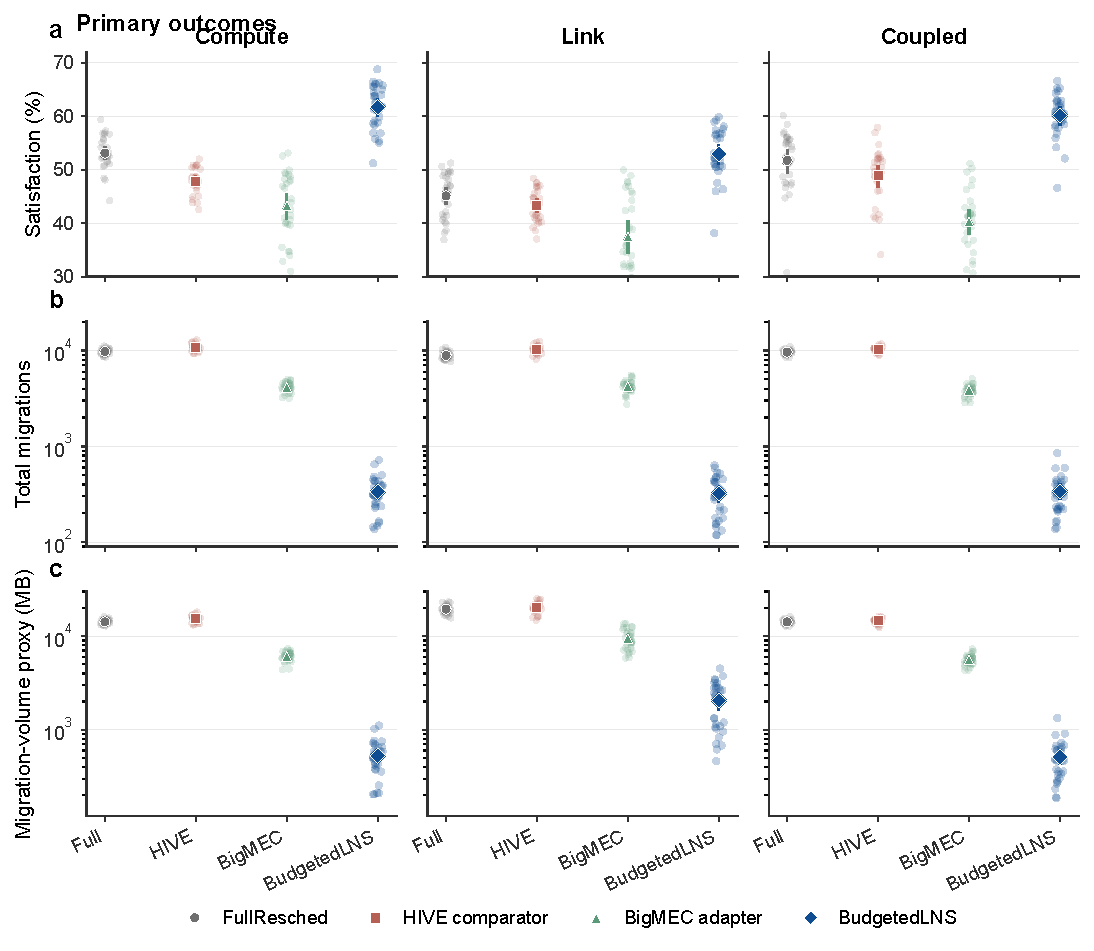
\includegraphics{Fig2.pdf}
\caption{Primary service, admitted-to-admitted node-change, and migration-volume-proxy outcomes. The node-change and volume measures exclude admission and rejection transitions. Panel (a) uses a linear satisfaction axis; panels (b) and (c) use logarithmic vertical axes, so equal vertical distances represent equal ratios, not equal absolute differences. Exact arithmetic means appear in Table~\ref{tab:main-results}.}
\end{figure}

\subsection{Synthetic event and relative-convergence results}\label{synthetic-event-recovery-results}

Table~\ref{tab:synthetic-event-results} reports event-minus-control satisfaction
differences in percentage points, averaged over the ten event slots and then
over 30 paired seeds. The results include negative, near-zero, and positive
effects. Node failure produces the clearest degradation in this simulator,
whereas jitter and concurrent pressure can be near zero or positive under some
background states. BudgetedLNS is therefore not uniformly superior across
interventions. These are descriptive, simulator-specific mean effects and do
not establish general fault tolerance.

\begin{table}[t]
\centering
\caption{Formal synthetic event effects. $\Delta S$ is the event-minus-control mean satisfaction difference in percentage points. Each value averages 30 paired seeds.}\label{tab:synthetic-event-results}
\small
\resizebox{\linewidth}{!}{%
\begin{tabular}{llrr}
\toprule
Background & Event & FullResched $\Delta S$ & BudgetedLNS $\Delta S$ \\
\midrule
Compute & Node failure & $-29.519$ & $-24.506$ \\
Compute & Network jitter & $-0.102$ & $+1.565$ \\
Compute & Migrating hotspot & $-10.759$ & $-11.035$ \\
Compute & Concurrent hotspots & $+0.887$ & $+0.322$ \\
Link & Node failure & $-24.730$ & $-21.757$ \\
Link & Network jitter & $+0.528$ & $+0.302$ \\
Link & Migrating hotspot & $-2.833$ & $+0.511$ \\
Link & Concurrent hotspots & $+0.224$ & $-1.241$ \\
Coupled & Node failure & $-29.098$ & $-23.693$ \\
Coupled & Network jitter & $-0.448$ & $+0.117$ \\
Coupled & Migrating hotspot & $-6.819$ & $-6.744$ \\
Coupled & Concurrent hotspots & $+0.661$ & $+2.487$ \\
\bottomrule
\end{tabular}%
}
\end{table}

Table~\ref{tab:relative-convergence} reports the relative-convergence
distribution for both methods. The event-window means in Table~\ref{tab:synthetic-event-results}
summarize slots 26--35, whereas the convergence measure evaluates the
event--control gap from slot 36, after the event has ended. Thus, a zero-delay
crossing can coexist with a large event-window loss: it means only that the
event and control arms meet the tolerance at the first post-event observation,
not that service has returned to its pre-event level. The median is conditional
on an observed crossing; non-crossings by slot 100 are shown separately. Many
cells cross at delay zero, including cells with little or no measured
post-event gap. The indicator therefore does not measure absolute service
restoration. In particular, node-failure runs under BudgetedLNS have censored
crossings in 11/30 compute-background seeds, 1/30 link-background seed, and
6/30 coupled-background seeds.

\begin{table}[t]
\centering
\caption{Exploratory event--control relative-convergence delays, counted from the first post-event observation at slot 36. Entries give observed crossings/30; median slots [interquartile range] among observed crossings. Non-crossings by slot 100 are censored and reported in parentheses. Zero means the tolerance is met at the first observation slot; it does not mean absolute service restoration.}\label{tab:relative-convergence}
\scriptsize
\resizebox{\linewidth}{!}{%
\begin{tabular}{llrr}
\toprule
Background & Event & FullResched & BudgetedLNS \\
\midrule
Compute & Node failure & 30/30; 0 [0, 0] & 19/30; 12 [9, 24.5] (11 censored) \\
Compute & Network jitter & 30/30; 0 [0, 0] & 30/30; 0 [0, 1] \\
Compute & Migrating hotspot & 30/30; 0 [0, 0] & 30/30; 0 [0, 0.8] \\
Compute & Concurrent hotspots & 30/30; 0 [0, 0] & 30/30; 0 [0, 0] \\
Link & Node failure & 30/30; 0 [0, 0] & 29/30; 3 [0, 15] (1 censored) \\
Link & Network jitter & 30/30; 0 [0, 0] & 30/30; 0 [0, 0] \\
Link & Migrating hotspot & 30/30; 0 [0, 0] & 30/30; 0 [0, 0] \\
Link & Concurrent hotspots & 30/30; 0 [0, 0] & 30/30; 0 [0, 0.8] \\
Coupled & Node failure & 30/30; 0 [0, 0] & 24/30; 11 [9, 18.8] (6 censored) \\
Coupled & Network jitter & 30/30; 0 [0, 0] & 30/30; 0 [0, 0.8] \\
Coupled & Migrating hotspot & 30/30; 0 [0, 0] & 29/30; 0 [0, 0] (1 censored) \\
Coupled & Concurrent hotspots & 30/30; 0 [0, 0] & 30/30; 0 [0, 1.8] \\
\bottomrule
\end{tabular}%
}
\end{table}

The accompanying exploratory logical access-interruption study produced event-
minus-control satisfaction differences of $-9.241$ and $-6.696$ percentage
points for FullResched and BudgetedLNS in the compute background, $-5.139$ and
$-6.369$ in the link background, and $-6.165$ and $-2.596$ in the coupled
background. BudgetedLNS crossed the exploratory relative-convergence tolerance
in 28/30, 28/30, and 30/30 seeds, respectively; FullResched crossed in 30/30
seeds in all three backgrounds. These crossings do not establish absolute
service restoration. The results are limited to logical task--node
reachability and are not evidence of physical link-disconnection recovery.
Flash-crowd surges
remain untested because no dynamic arrival process is present in the simulator.

\subsection{Implemented hierarchical comparator}\label{implemented-hierarchical-comparator}

The matched HIVE comparator exhibits lower mean satisfaction and
substantially higher admitted-to-admitted node-change counts in every tested
persistent-hotspot cell. BudgetedLNS has a 9.65--13.82-point satisfaction
advantage and 96.74--96.88\% fewer such changes (Figure 3). Against the code-derived
BigMEC adapter, the corresponding advantages are 15.49--19.92 points and
91.21--92.36\% fewer admitted-to-admitted node changes. These are bounded comparator comparisons,
without extending the claims to the complete BigMEC system or to untested
hierarchical or learned controllers.

\begin{figure}[!htbp]
\centering
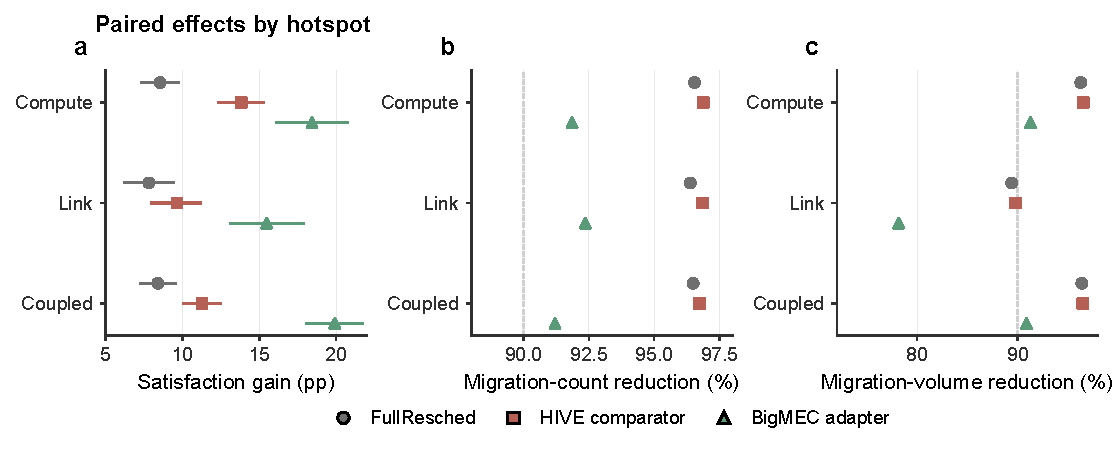
\includegraphics{Fig3.pdf}
\caption{Paired effects against the implemented comparators. Migration-count reduction means reduction in admitted-to-admitted node changes; migration-volume reduction is the profile-derived \texttt{MigrationMB} proxy.}
\end{figure}

\subsection{Hotspot onset and persistence}
\label{hotspot-onset}

The onset experiment starts from a normal, feasible deployment for slots
1--50 and introduces the selected compute, link, or coupled hotspot at
slot 51, after which the condition is maintained through slot 200. The
slot-level trajectories in Figure 4 therefore show the post-onset response
rather than a cold-start stress test. Across the three onset cells,
BudgetedLNS improves post-onset satisfaction over the slot-wise MPC rollout
comparator by
8.77--9.95 percentage points and reduces post-onset admitted-to-admitted
node changes by 96.49--97.18\%. The corresponding HIVE-comparator gains
are 11.71--15.21 points and 96.73--97.52\% fewer admitted-to-admitted node
changes. These paired effects use the
same 30 onset seeds and should be interpreted only for the specified
slot-51 intervention.

\begin{figure}[!htbp]
\centering
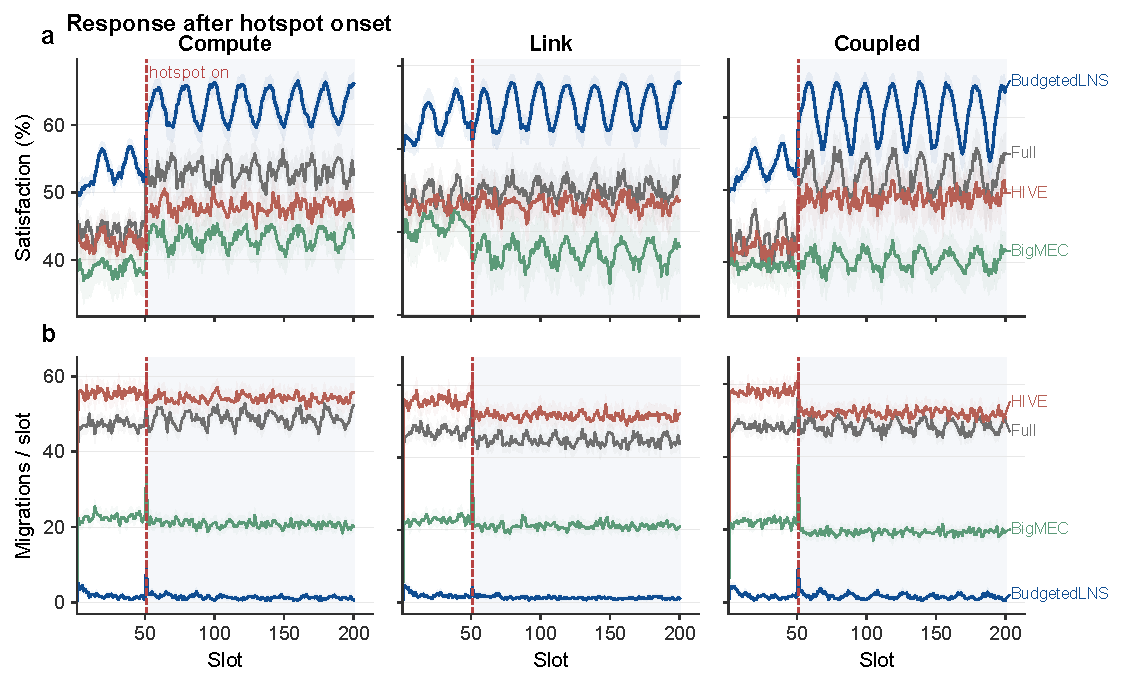
\includegraphics{Fig4.pdf}
\caption{Hotspot-onset response after a feasible warm-up. Migration traces count admitted-to-admitted node changes; admission and rejection transitions are excluded.}
\end{figure}

\subsection{Component ablation}
\label{component-ablation}

The component comparison keeps the common inputs, repair, and metrics
fixed. Figure 5 shows the earlier slot-51 contrasts from 30 paired runs per
hotspot profile; these are separate from the new 90-pair formal ablation in
Table~\ref{tab:core-audit-ablation}. Relative to the full method, cold start
reduced post-onset satisfaction by 8.77--9.95 percentage points and increased
node changes from 191--255 to 6,710--7,336 per run. The global-pool variant
increased satisfaction by 4.02--5.43 points (negative full-minus-variant
values in Figure 5a) and increased node changes from 191--255 to 325--462
per run. This global-pool contrast jointly removes pressure localization and
the 3B cap, so its effects cannot be attributed to either factor alone. The
new formal ablation separates these factors and also compares the proposed
lexicographic acceptance rule with a fixed weighted-sum rule. Across the 90 paired
scenario/run cells, the weighted-sum variant reduces mean satisfaction by
6.96 percentage points (95\% CI [6.07, 7.85] for the magnitude of the
decrease) and reduces admitted-to-admitted changes, showing that a single
scalar score does not preserve the proposed service-first ordering. Removing
the (3B) cap increases satisfaction by 3.05 percentage points but adds
28,397 evaluator calls per run on average and increases solver time by
24.79 s per 200-slot run. This is a computation--service trade-off, not a
free performance gain. Removing pressure localization decreases satisfaction
by 2.07 points and increases admitted-to-admitted changes by 208.12 per run.
Removing the trial-level guard changes mean satisfaction by only -0.09 points
and the migration count by -4.23 changes per run; the guard is therefore
primarily an auditability and controllability mechanism in these cells, not a
large satisfaction mechanism. The onset contrasts in Figure 5 and the formal component estimates in
Table~\ref{tab:core-audit-ablation} answer different questions and are not
pooled.

\begin{table}[H]
\centering
\caption{Formal paired component ablation over 90 scenario/run pairs. Deltas are variant minus BudgetedLNS; sat. denotes satisfaction, changes denotes admitted-to-admitted node changes, eval. denotes evaluator calls, and time is solver runtime.}
\label{tab:core-audit-ablation}
\scriptsize
\begin{tabular}{lrrrr}
\toprule
Variant & $\Delta$ sat. (pp) & $\Delta$ changes & $\Delta$ eval. & $\Delta$ time (s) \\
\midrule
Weighted-sum & -6.96 & -203.74 & +14.68 & +1.00 \\
No-$3B$ cap & +3.05 & -0.17 & +28,396.53 & +24.79 \\
No top-$K$ localization & -2.07 & +208.12 & -13.22 & +0.29 \\
No guard & -0.09 & -4.23 & +169.56 & +0.09 \\
\bottomrule
\end{tabular}
\end{table}

\subsection{True local-search-off ablation}
\label{local-search-off-ablation}

To isolate the contribution of the local-search procedure itself, we added a
paired variant named \texttt{LNSNoLocalSearch}. It uses the same current-slot
revalidation, common feasibility repair, final reporting evaluator, task
inputs, seeds, and paired protocol as \texttt{BudgetedLNS}, but skips candidate-pool
construction, trial generation, acceptance, and all inner updates. Its
local-search invocation, inner-update, candidate-evaluation, and accepted-move
counters are zero by construction. This is a mechanism ablation rather than
an equal-compute or equal-wall-time comparison, because the enabled method
performs additional simulator work.

The formal run contains three hotspot profiles, 30 paired runs per profile,
180 tasks, and 200 slots. The complete replay has 360 run-level rows and
72,000 slot-level rows; all resource-violation rates are zero and all
run-level summaries reconstruct from the slot-level traces.

\subsection{Local-search contribution and cost}
\label{local-search-results}

The true local-search-off replay supports a positive satisfaction contribution
under the tested simulator protocol. Relative to \texttt{LNSNoLocalSearch},
\texttt{BudgetedLNS} improves mean satisfaction by 9.30 percentage points
in the compute-hotspot profile, 13.60 points in the link-hotspot profile, and
10.98 points in the coupled-hotspot profile; all three paired sign-flip tests
have $p<10^{-4}$. The effect is not a universal migration reduction. Mean
admitted-to-admitted node changes are higher with local search in all three
profiles, while the \texttt{MigrationMB} proxy is higher in compute and coupled
hotspots and slightly lower, without a significant paired difference, in the
link-hotspot profile ($p=0.741$).

The enabled method also incurs a substantial simulator cost: mean solver
runtime is 21.31--24.25 s per 200-slot run versus 0.139--0.170 s for the
off variant, and it performs about 21,396--21,481 additional candidate
evaluations per run. These values are MATLAB simulator timings and counters,
not deployment latency or an equal-compute fairness result. The ablation
therefore supports a bounded claim: local search improves service in these
persistent-hotspot cells at a measurable computational and, in some profiles,
reconfiguration cost. It does not justify presenting local search as a
mechanism that uniformly minimizes migration.

\begin{table}[H]
\centering
\caption{True local-search-off ablation over 30 paired runs per hotspot profile. Differences are BudgetedLNS minus LNSNoLocalSearch. Runtime and candidate counts are simulator-level measures.}
\label{tab:local-search-off}
\scriptsize
\setlength{\tabcolsep}{4pt}
\begin{tabular}{lrrrrrr}
\toprule
Profile & $\Delta$ sat. (pp) & $\Delta$ changes & $\Delta$ volume (MB) & LNS time (s) & Off time (s) & LNS eval. \\\\
\midrule
Compute & +9.30 & +196.03 & +280.07 & 22.13 & 0.149 & 21,421\\\\
Link & +13.60 & +155.57 & -85.33 & 21.31 & 0.139 & 21,481\\\\
Coupled & +10.98 & +244.87 & +384.74 & 24.25 & 0.170 & 21,396\\\\
\bottomrule
\end{tabular}
\end{table}

\subsection{Alternative SharedRepair order}
\label{alternative-repair-order}

To test sensitivity to the task-processing order used by the common feasibility repair, we ran a paired alternative-order ablation. The control retains the easy-first order, which processes tasks by ascending minimum computation time across nodes. The alternative uses earliest-deadline-first; deterministic task-index order breaks ties. All other repair rules, candidate pools, solver streams, local-search settings, and input traces are unchanged.

Across 90 paired scenario/run cells, earliest-deadline-first reduced mean satisfaction by 0.726 percentage points (95\% CI [-1.028, -0.431]), increased admitted-to-admitted changes by 283.3 per 200-slot run (95\% CI [257.5, 309.5]), and increased the profile-derived migration volume by 943.1 MB (95\% CI [759.9, 1134.0]). Mean admitted tasks differed by only 0.011 (95\% CI [-0.015, 0.037]). The satisfaction effect was -1.143 points for compute hotspots, -0.765 points for coupled hotspots, and -0.269 points for link hotspots; the link-hotspot interval included zero.

The alternative also produced 228 repair-overridden slots versus 103 for the control; the maximum observed budget excess was 11 versus 10. Both arms had zero resource violations. These results indicate sensitivity to repair order under the present simulator and persistent-hotspot protocol. They do not establish a generally optimal order, and the alternative is therefore reported as a negative/neutral sensitivity result rather than as an improvement. Runtime is excluded from this comparison because the run logs contain extreme outliers and the protocol does not impose a separately controlled wall-time budget.

\begin{table}[H]
\centering
\caption{Alternative SharedRepair order ablation over 90 paired scenario/run cells. Deltas are earliest-deadline-first minus the easy-first control.}
\label{tab:alternative-repair}
\scriptsize
\begin{tabular}{lrrr}
\toprule
Metric & Mean delta & 95\% CI low & 95\% CI high \\
\midrule
Mean satisfaction (pp) & -0.726 & -1.028 & -0.431 \\
Admitted-to-admitted changes & +283.3 & +257.5 & +309.5 \\
Migration volume (MB) & +943.1 & +759.9 & +1134.0 \\
Mean admitted tasks & +0.011 & -0.015 & +0.037 \\
\bottomrule
\end{tabular}
\end{table}

\subsection{Alternative fallback feasibility rule}\label{alternative-feasibility-rule}

The task-order comparison above keeps the feasibility contract fixed. To test a repair change that directly alters feasibility, we compared the current fallback rule with a deadline-strict fallback in a separate paired replay. Both policies first retain the input node when its existing memory, normalized-load, and insertion-time latency checks pass. If retention fails, the current policy selects the feasible fallback with the lowest calculated insertion-time latency; the strict policy considers only fallback nodes whose calculated latency is no greater than the task deadline, rejecting the task if no such node exists. Task order, solver, candidate pool, local-search settings, seeds, traces, and terminal evaluator were held fixed. We ran 30 paired seeds for each of the three hotspot scenarios (compute, link, and coupled), with 180 tasks and 200 slots per run, for both BudgetedLNS and FullResched.

Table~\ref{tab:alternative-feasibility-rule} reports paired mean differences (deadline-strict minus current) for each scenario and solver. The strict fallback increased mean satisfaction and reduced accumulated admitted-task deadline-miss events in all six contrasts. It also admitted slightly fewer tasks per slot. These are descriptive paired results for this simulator and protocol; we do not interpret them as a universal policy ranking or a hard deadline guarantee. Deadline misses remain possible after later insertions and are counted separately. Resource-violation rows were zero in both policies.

The budget audit also shows why the 5\% local-search budget is not an absolute bound on delivered inter-slot migrations. Among 18,000 BudgetedLNS slots per policy, inter-slot budget-excess events occurred in 103 current-policy slots and 68 deadline-strict slots. An event means that observed admitted-to-admitted node changes exceeded the recorded move budget after current-slot revalidation and repair; it does not attribute the excess solely to terminal repair. The maximum per-slot excess was 10 and 8 moves, respectively. We report these events explicitly and retain the distinction between a local-trial guard and total delivered placement changes.

\begin{table}[H]
\centering
\caption{Paired effect of deadline-strict fallback repair relative to the current fallback policy. Each row summarizes 30 paired seeds; differences are strict minus current. Sat. = satisfaction (percentage points); Admit = mean admitted tasks per slot; Miss = admitted-task deadline-miss events summed over 200 slots (not unique tasks); Moves = admitted-to-admitted node changes per run.}
\label{tab:alternative-feasibility-rule}
\scriptsize
\setlength{\tabcolsep}{3pt}
\begin{tabular}{llrrrr}
\toprule
Scenario & Solver & $\Delta$ Sat. & $\Delta$ Admit/slot & $\Delta$ Miss/run & $\Delta$ Moves/run \\
\midrule
Compute & BudgetedLNS & +0.689 & -0.067 & -261.4 & -53.2 \\
Compute & FullResched & +1.407 & -0.119 & -530.4 & -147.0 \\
Link & BudgetedLNS & +2.251 & -0.288 & -868.0 & -39.8 \\
Link & FullResched & +1.281 & -0.050 & -471.3 & -131.0 \\
Coupled & BudgetedLNS & +1.463 & -0.181 & -562.7 & -40.1 \\
Coupled & FullResched & +1.210 & -0.091 & -453.9 & -154.3 \\
\bottomrule
\end{tabular}
\end{table}

\subsection{Controlled scale check}\label{controlled-scale-check}

The 20-node/500-task check comprises 30 matched seed/profile pairs (10 seeds for each of three hotspot profiles) and 90 method records (three methods per pair); all records passed resource and duplicate-slot checks. BudgetedLNS achieved 89.92\% mean
satisfaction versus 89.35\% for FullResched and 76.07\% for the BigMEC
adapter. It recorded 130.63 admitted-to-admitted changes per 100-slot run,
compared with 28,642.03 for FullResched and 15,613.43 for the BigMEC adapter.
The corresponding solver times were 110.39, 11.49, and 0.26 s per run,
respectively. These timings are simulator solver timings under the controlled
protocol; they are not real migration latency or production control-plane
latency. The result supports a limited transfer of the mechanism to this
synthetic 20-node/500-task configuration, but not the full requested scale or
topology generalization.

\begin{table}[H]
\centering
\caption{Controlled 20-node/500-task scale check. Ten paired runs were used for each of three persistent-hotspot profiles.}
\label{tab:scale-check}
\scriptsize
\begin{tabular}{lrrr}
\toprule
Method & Satisfaction (\%) & Admitted-to-admitted changes & Solver time (s/run) \\
\midrule
FullResched & 89.35 & 28,642.03 & 11.49 \\
BigMEC adapter & 76.07 & 15,613.43 & 0.26 \\
BudgetedLNS & 89.92 & 130.63 & 110.39 \\
\bottomrule
\end{tabular}
\end{table}

\subsubsection{Independent 20-node/750-task scale audit} An independent scale audit increased the synthetic configuration to 750 tasks and retained 20 heterogeneous nodes, 200 slots, three persistent-hotspot profiles, 30 paired runs per profile, the same evaluator and repair contract, and the frozen 5\% local budget. This audit used FullResched and BudgetedLNS; it was not pooled with the primary $N=180$ release or with the separate 20-node/500-task check. All 36,000 slot rows passed duplicate-key, resource-feasibility, admission-conservation, and run-level reconstruction checks. Mean satisfaction was 68.72\%/68.78\%/69.75\% for BudgetedLNS and 62.69\%/63.24\%/60.34\% for FullResched in compute, coupled, and link profiles, respectively. Across the 30 paired seeds, the satisfaction differences (BudgetedLNS minus FullResched) were +6.02, +5.54, and +9.41 percentage points, with 95\% paired t intervals [5.68, 6.36], [5.13, 5.94], and [8.96, 9.86]; BudgetedLNS had higher satisfaction in 30/30 pairs in each profile. The corresponding admitted-to-admitted node-change counts were 35.20/36.60/73.53 and 70,163.90/70,113.77/71,577.60 per 200-slot run. BudgetedLNS therefore incurred about 14--15 times the simulator solver time of FullResched in this scale audit, a material cost that accompanies the satisfaction and node-change differences. These simulator outputs provide a controlled scale check and do not establish full topology generality, physical migration latency, control-plane traffic, or deployment-level cost.  \begin{table}[H] \centering \caption{Paired satisfaction results for the independent synthetic 20-node/750-task scale audit. Values are means over 30 paired runs per profile. Differences are BudgetedLNS minus FullResched with paired 95\% t confidence intervals.} \label{tab:scale-audit-750-service} \small \begin{tabular}{llrr} \toprule Profile & Method & Satisfaction (\%) & Paired difference (\textit{pp}, 95\% CI) \\ \midrule Compute & FullResched & 62.69 & -- \\ Compute & BudgetedLNS & 68.72 & +6.02 [5.68, 6.36] \\ Coupled & FullResched & 63.24 & -- \\ Coupled & BudgetedLNS & 68.78 & +5.54 [5.13, 5.94] \\ Link & FullResched & 60.34 & -- \\ Link & BudgetedLNS & 69.75 & +9.41 [8.96, 9.86] \\ \bottomrule \end{tabular} \end{table}   \begin{table}[H] \centering \caption{Reconfiguration and simulator solver-time means for the independent 20-node/750-task scale audit; each value averages 30 paired runs of 200 slots.} \label{tab:scale-audit-750-cost} \small \begin{tabular}{llrr} \toprule Profile & Method & Node changes/run & Solver time (s/run) \\ \midrule Compute & FullResched & 70,163.90 & 37.92 \\ Compute & BudgetedLNS & 35.20 & 528.32 \\ Coupled & FullResched & 70,113.77 & 38.94 \\ Coupled & BudgetedLNS & 36.60 & 562.45 \\ Link & FullResched & 71,577.60 & 36.24 \\ Link & BudgetedLNS & 73.53 & 527.45 \\ \bottomrule \end{tabular} \end{table} \subsubsection{Independent 50-node/2,000-task scale endpoint}
We ran a separate short-horizon synthetic endpoint with 50 heterogeneous nodes,
2,000 tasks, 10 slots, three persistent-hotspot profiles, and 10 matched seed
pairs per profile. It compares only FullResched and BudgetedLNS and uses the
same evaluator, repair contract, and frozen 5\% local budget. The 60 run-level
and 600 slot-level rows passed duplicate-key, seed-pair, admission-conservation,
zero resource-violation, exact-slot-coverage, and run-to-slot reconstruction
checks. Mean satisfaction for FullResched versus BudgetedLNS was 62.86\% versus
64.64\% (compute), 61.63\% versus 65.25\% (link), and 62.82\% versus 64.87\%
(coupled). Paired differences were +1.78 [95\% CI: 1.52, 2.05], +3.62
[3.17, 4.06], and +2.05 [1.73, 2.37] percentage points, respectively;
BudgetedLNS was higher in all 10 paired runs per profile. Its accumulated
admitted-to-admitted node changes were lower by 99.72--99.82\% in this short
horizon. Simulator solver time was approximately 16.8--17.0 times that of
FullResched. These paired intervals are descriptive and unadjusted for multiple
profile/metric comparisons.

This endpoint supports only a limited statement that the implemented method
ran at this synthetic scale under the stated 10-slot protocol. It does not test
long-horizon behavior, topology variation, uniform/tree/San Francisco BigMEC
networks, external SOTA methods, physical migration cost, or deployment-level
performance; it is not combined with the 20-node audits or the primary release.
\begin{table}[H]\centering
\caption{Paired results for the independent synthetic 50-node/2,000-task, 10-slot endpoint (10 matched seeds per profile). Satisfaction differences are BudgetedLNS minus FullResched with descriptive paired 95\% t intervals.}
\label{tab:scale-audit-2000-service}\scriptsize\setlength{\tabcolsep}{3pt}
\begin{tabular}{lrrrr}\toprule
Profile & Full satisfaction (\%) & BudgetedLNS (\%) & Difference (pp) & 95\% CI \\ \midrule
Compute & 62.86 & 64.64 & +1.78 & [1.52, 2.05] \\
Link & 61.63 & 65.25 & +3.62 & [3.17, 4.06] \\
Coupled & 62.82 & 64.87 & +2.05 & [1.73, 2.37] \\ \bottomrule\end{tabular}\end{table}
\begin{table}[H]\centering
\caption{Admitted-to-admitted changes and simulator solver time for the independent 50-node/2,000-task, 10-slot endpoint; means over 10 paired runs.}
\label{tab:scale-audit-2000-cost}\scriptsize\setlength{\tabcolsep}{3pt}
\begin{tabular}{lrrrrr}\toprule
Profile & Full changes & BudgetedLNS changes & Reduction (\%) & Full time (s) & BudgetedLNS time (s) \\ \midrule
Compute & 9,204.50 & 16.60 & 99.82 & 14.60 & 245.43 \\
Link & 9,308.20 & 21.60 & 99.77 & 13.77 & 234.05 \\
Coupled & 9,212.30 & 26.20 & 99.72 & 13.80 & 231.84 \\ \bottomrule\end{tabular}\end{table}

\subsubsection{Separate graph-topology sensitivity}

The graph-topology replay passed the row, pairing, resource-feasibility, and
run-to-slot reconstruction checks for 9,000 slot rows and 180 run records.
Across 30 paired seeds, the mean satisfaction difference
(\texttt{BudgetedLNS} minus \texttt{FullResched}) was +0.80 percentage points
for the BigMEC-derived San Francisco geometry, +2.79 for uniform Delaunay,
and +3.95 for the uniform tree. The paired differences were positive in 8,
26, and 30 seeds, respectively; all other pairs were ties and none were
negative. The intervals in Table~\ref{tab:topology-sensitivity-service} are
unadjusted paired t 95\% intervals, while the reported sign-flip tests are
Holm-adjusted across the three topology comparisons.

The satisfaction differences do not demonstrate migration reduction: mean
admitted-to-admitted changes per 50-slot run were 0/0 for both methods on the
first two graphs and 0/1 on the tree. Deadline-violation rates were nonzero,
and BudgetedLNS used substantially more simulator solver time and evaluator
calls per slot. These outcomes are reported together in
Table~\ref{tab:topology-sensitivity-cost}. The replay is therefore a limited
topology/evaluator sensitivity result at one scale point, not evidence of
long-horizon hotspot robustness, migration benefit, equal-compute fairness,
or a real San Francisco MEC deployment.

\begin{table}[H]\centering
\caption{Separate 20-node/500-task graph-topology sensitivity replay. Satisfaction means are over 30 paired 50-slot runs per topology; F/B denote FullResched/BudgetedLNS. The difference is BudgetedLNS minus FullResched; intervals are unadjusted paired t 95\% confidence intervals. The p-values use paired two-sided sign-flip tests with Holm adjustment across the three topology comparisons.}\label{tab:topology-sensitivity-service}
\scriptsize\setlength{\tabcolsep}{3pt}\renewcommand{\arraystretch}{1.12}
\begin{tabular}{lcccc}\toprule
Topology & Satisfaction F/B (\%) & Difference (pp; 95\% CI) & Positive/tied & Holm $p$ \\ \midrule
SF-derived Delaunay & 94.82 / 95.62 & +0.80 [0.30, 1.30] & 8 / 22 & 0.00766 \\
Uniform Delaunay & 94.58 / 97.37 & +2.79 [2.33, 3.24] & 26 / 4 & $3.0\times10^{-5}$ \\
Uniform MST tree & 82.12 / 86.07 & +3.95 [3.29, 4.62] & 30 / 0 & $3.0\times10^{-5}$ \\
\bottomrule\end{tabular}
\end{table}

\begin{table}[H]\centering
\caption{Feasibility, movement, and simulator work for the graph-topology sensitivity replay. Values are means over 30 seeds; F/B denote FullResched/BudgetedLNS. Solver time and evaluator calls are per slot.}\label{tab:topology-sensitivity-cost}
\scriptsize\setlength{\tabcolsep}{3pt}\renewcommand{\arraystretch}{1.12}
\begin{tabular}{lcccc}\toprule
Topology & \shortstack{Deadline viol.\\F/B (\%)} & \shortstack{Node changes/run\\F/B} & \shortstack{Solver (s/slot)\\F/B} & \shortstack{Evaluator calls/slot\\F/B} \\ \midrule
SF-derived Delaunay & 5.18 / 4.38 & 0.00 / 0.00 & 0.108 / 1.205 & 1 / 915.65 \\
Uniform Delaunay & 5.42 / 2.63 & 0.00 / 0.00 & 0.108 / 1.215 & 1 / 932.10 \\
Uniform MST tree & 17.88 / 13.93 & 0.00 / 1.00 & 0.108 / 1.527 & 1 / 1,038.52 \\
\bottomrule\end{tabular}
\end{table}

\subsubsection{Crossed static scale--topology results}

The scale--topology matrix contains 540 method-condition rows (three selected
scale pairs, three graphs, 30 seeds, and two methods). All pairs are complete,
admission counts sum to the task count, resource-violation rates are zero, and
the stored summaries reconstruct from the slot records. The mean paired
satisfaction differences (\texttt{BudgetedLNS} minus \texttt{FullResched})
range from +0.25 to +3.63 percentage points (Table~\ref{tab:static-scale-topology-service});
the magnitude depends on graph and scale. In the BigMEC-derived Delaunay cells,
only 7--8 of 30 pairs were strictly positive and 22--23 were ties. The
synthetic MST cells show larger paired differences, but their absolute
satisfaction is lower, reaching 45.46\% versus 47.03\% at 50 nodes/2,000
tasks. All nine paired 95\% t intervals exclude zero, and the two-sided
Monte Carlo sign-flip tests remain below 0.05 after Holm adjustment across
the nine conditions; these tests do not remove the practical heterogeneity
between graphs.

The service differences have a measurable solver-time cost. Across these
one-slot cells, the mean simulator solver time for \texttt{BudgetedLNS} is
13.9--26.1 times that of \texttt{FullResched} (Table~\ref{tab:static-scale-topology-cost});
these are solver-call timings, not equal-compute comparisons or deployment
latencies. Deadline violations range from 2.63\% to 54.54\% and remain high
in the largest synthetic MST condition, so the positive satisfaction
difference must not be read as deadline compliance. Resource violations are
zero, but deadline feasibility is not guaranteed. The one-slot protocol
contains no temporal reconfiguration contrast and therefore supports no
migration-reduction claim. These results extend static simulator coverage
across the tested scale pairs and graphs only; they do not test persistent
hotspots at $M>20$, a long horizon at the largest scale, or a deployed San
Francisco MEC network.

\begin{table}[htbp]\centering
\caption{Crossed static scale--topology satisfaction matrix. Each scale pair has 30 paired seeds and one decision slot per seed; the $(20,500)$ rows reuse slot 1 of the separate 50-slot graph replay. F/B denote \texttt{FullResched}/\texttt{BudgetedLNS}. Differences are paired means with unadjusted paired 95\% $t$ intervals. Holm $p$ values use two-sided Monte Carlo sign-flip tests with 100,000 sign assignments per condition, adjusted across nine conditions.}\label{tab:static-scale-topology-service}
\scriptsize\setlength{\tabcolsep}{2pt}\renewcommand{\arraystretch}{1.10}
\begin{tabular}{llcccc}\toprule
Topology & $M/N$ & Satisfaction F/B (\%) & Difference (pp; 95\% CI) & Positive/tied & Holm $p$ \\ \midrule
SF-derived Delaunay & 20/500 & 94.82 / 95.62 & +0.80 [0.30, 1.30] & 8/22 & 0.0219 \\
SF-derived Delaunay & 30/750 & 94.32 / 94.57 & +0.25 [0.09, 0.41] & 8/22 & 0.0219 \\
SF-derived Delaunay & 50/2000 & 65.76 / 66.19 & +0.43 [0.13, 0.73] & 7/23 & 0.0219 \\
Uniform Delaunay & 20/500 & 94.58 / 97.37 & +2.79 [2.33, 3.24] & 26/4 & $9.0\times10^{-5}$ \\
Uniform Delaunay & 30/750 & 94.25 / 96.37 & +2.12 [1.91, 2.33] & 29/1 & $9.0\times10^{-5}$ \\
Uniform Delaunay & 50/2000 & 65.73 / 66.53 & +0.80 [0.42, 1.19] & 12/18 & 0.0026 \\
Uniform MST tree & 20/500 & 82.12 / 85.75 & +3.63 [2.98, 4.29] & 30/0 & $9.0\times10^{-5}$ \\
Uniform MST tree & 30/750 & 82.83 / 86.13 & +3.31 [2.97, 3.64] & 30/0 & $9.0\times10^{-5}$ \\
Uniform MST tree & 50/2000 & 45.46 / 47.03 & +1.57 [1.25, 1.89] & 30/0 & $9.0\times10^{-5}$ \\
\bottomrule\end{tabular}
\end{table}

\begin{table}[htbp]\centering
\caption{Deadline violations and simulator solver time in the crossed static scale--topology matrix. Values are means over 30 paired seeds; F/B denote \texttt{FullResched}/\texttt{BudgetedLNS}. Solver times are per decision slot. All method-condition rows had zero resource violations.}\label{tab:static-scale-topology-cost}
\scriptsize\setlength{\tabcolsep}{4pt}\renewcommand{\arraystretch}{1.10}
\begin{tabular}{llcc}\toprule
Topology & $M/N$ & Deadline violations F/B (\%) & Solver time F/B (s/slot) \\ \midrule
SF-derived Delaunay & 20/500 & 5.18 / 4.38 & 0.111 / 1.544 \\
SF-derived Delaunay & 30/750 & 5.68 / 5.43 & 0.330 / 4.637 \\
SF-derived Delaunay & 50/2000 & 34.24 / 33.81 & 2.113 / 45.222 \\
Uniform Delaunay & 20/500 & 5.42 / 2.63 & 0.109 / 1.785 \\
Uniform Delaunay & 30/750 & 5.75 / 3.63 & 0.478 / 7.566 \\
Uniform Delaunay & 50/2000 & 34.27 / 33.47 & 2.044 / 45.495 \\
Uniform MST tree & 20/500 & 17.88 / 14.25 & 0.109 / 1.857 \\
Uniform MST tree & 30/750 & 17.17 / 13.87 & 0.362 / 6.694 \\
Uniform MST tree & 50/2000 & 54.54 / 52.97 & 1.944 / 50.752 \\
\bottomrule\end{tabular}
\end{table}

Figure 5 reports the component effects and the corresponding post-onset
migration volumes. The core ablation and scale-check results are controlled
simulator evidence rather than a universal causal decomposition or deployment
benchmark.

\begin{figure}[!htbp]
\centering
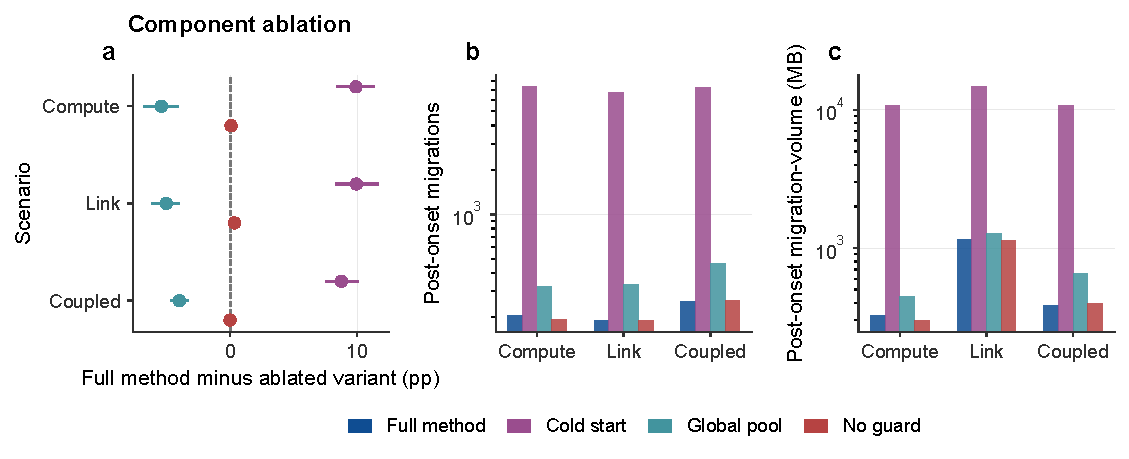
\includegraphics{Fig5.pdf}
\caption{Earlier slot-51 component contrasts (30 paired seeds per profile). Panel (a) plots full method minus variant; negative values mean the variant has higher satisfaction. Migration outcomes count admitted-to-admitted node changes, and volume is the profile-derived proxy.}
\end{figure}

\subsection{Bounded-search diagnostics}\label{bounded-search-diagnostics}

The frozen 5\% replay evaluates approximately 21.35k--21.49k candidates
per 200-slot run (106.75--107.46 evaluations per slot) and records
255.5--307.8 admitted-to-admitted node changes in the solver output. The 5\% local-search budget
is active in only 1.20--3.17 of 200 slots on average (Figure 6). Thus,
the observed savings do not arise from saturating the local-search
budget at every slot. Because admission and rejection remain
scenario-dependent, this diagnostic supports the bounded-search
interpretation but is not a causal decomposition of satisfaction gains.

We also ran an independent simulator profiling replay with 30 paired runs,
200 slots, three persistent-hotspot scenarios, and the three implemented
methods. The replay contains 54,000 slot records and 270 run records. Mean
solver-call wall time per slot was 0.0102~s for \texttt{FullResched},
0.0005~s for \texttt{BigMECGreedy}, and 0.0846~s for \texttt{BudgetedLNS};
the corresponding complete slot-pipeline means, including common repair,
final evaluation, and bookkeeping, were 0.0457, 0.0362, and 0.1199~s.
Evaluator, repair, and local-search times were recorded as inclusive component
diagnostics and are not additive. The run-level totals reconstruct exactly from
the slot-level records, paired seeds and task counts are identical, and all
reported resource-violation rates are zero. The memory field is a sampled
MATLAB heap value after the solver call, not peak process RSS. These measurements
provide simulator provenance only; they do not measure migration latency,
control-plane messages, hardware cost, or equivalent compute budgets.

\begin{figure}[!htbp]
\centering
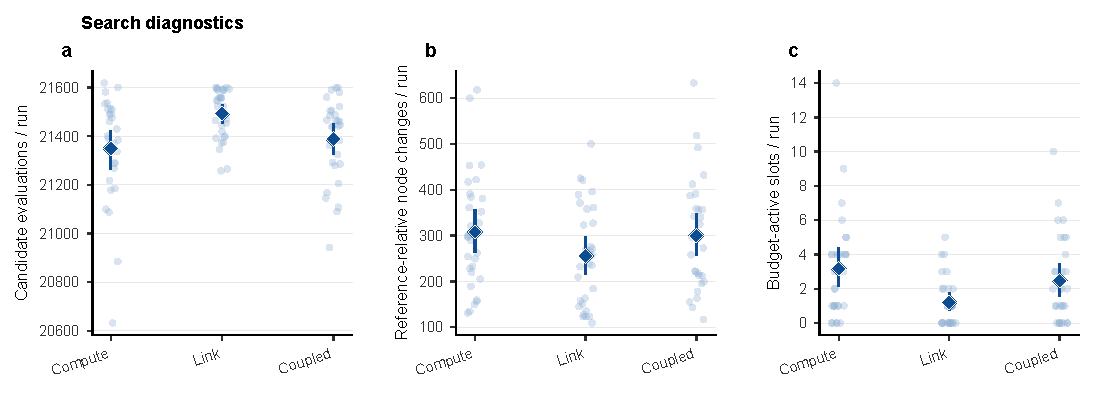
\includegraphics{Fig6.pdf}
\caption{Search diagnostics under the 5\% guard. The recorded reconfiguration quantity is the admitted-to-admitted node-change count in the solver output, not a complete placement-state transition count.}
\end{figure}

\subsection{Migration-budget boundary}\label{migration-budget-boundary}

The 1\%, 5\%, and 10\% sensitivity study isolates the budget parameter.
At 1\%, the local-search guard permits at most two admitted-to-admitted
node changes from the current-slot reference, while inter-slot counts
frequently exceed that threshold (15.97--26.17 excess events per run,
with maximum inter-slot excesses of 6--7 in the completed sensitivity cells). The
5\% primary cell still records a small number of inter-slot excess events (0.60--1.33
per run; maximum excess 3--6), while the 10\% cell has few inter-slot excess events
(0--0.10 per run; maximum excess 0--1). These are operating-point
diagnostics, not evidence of a universal absolute bound (Figure 7).

\subsection{Mobility-intensity sensitivity}\label{mobility-intensity-sensitivity}

We additionally varied the standard deviation of the existing independent
per-slot position jitter while holding the task mix, five-node environment,
hotspot profiles, paired seeds, evaluator, repair contract, and 5\% budget
fixed. The tested values were 15, 35, and 70~m. Table~\ref{tab:mobility-sensitivity}
reports paired BudgetedLNS-minus-FullResched satisfaction differences and
the reduction in total admitted-to-admitted node changes over each 200-slot
run. The intervals are percentile intervals from 20,000 paired bootstrap
resamples; they are descriptive and no p-values or universal trend are
claimed.

\begin{table}[!htbp]
\centering
\small
\caption{One-factor mobility-intensity sensitivity in the simulator. Each
cell summarizes the range across the compute, link, and coupled hotspot
profiles; each profile uses 30 paired seeds, 180 tasks, and 200 slots. The
mobility model independently resamples Gaussian jitter around initial
positions each slot.}
\label{tab:mobility-sensitivity}
\begin{tabular}{lcc}
\toprule
Jitter standard deviation & Satisfaction advantage (pp) & Migration reduction \\
\midrule
15~m & 7.39--8.25 & 96.98\%--97.37\% \\
35~m (frozen setting) & 7.82--8.55 & 96.39\%--96.55\% \\
70~m & 8.01--10.94 & 95.30\%--96.89\% \\
\bottomrule
\end{tabular}
\end{table}

The 35-m row reproduces the frozen primary protocol at all three profiles.
Across the tested jitter levels, the satisfaction advantage remained
positive and the migration reduction remained above 95\%, but the ranges
also changed with the jitter level and profile. This is evidence for the
tested one-factor simulator sensitivity only. It does not establish
robustness to real user trajectories, task-composition changes, or an
independently varied hotspot-severity dose.

\begin{figure}[!htbp]
\centering
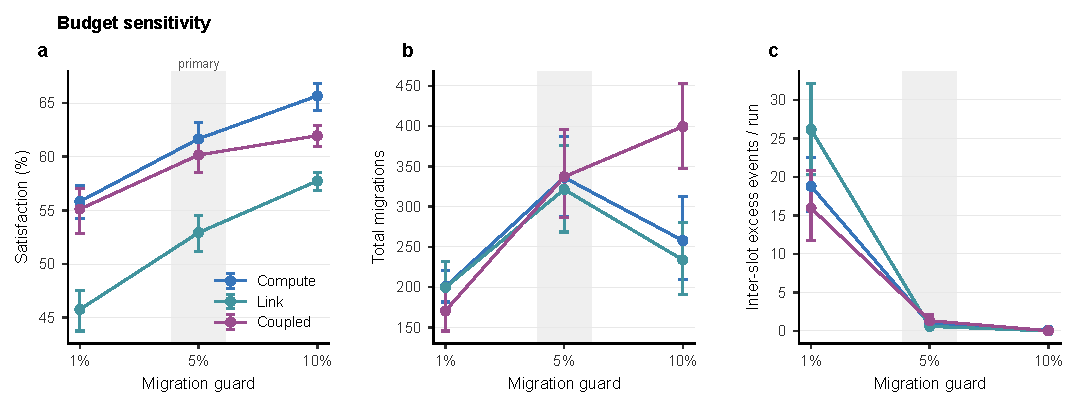
\includegraphics{Fig7.pdf}
\caption{Budget sensitivity and inter-slot budget excesses. Migration outcomes count admitted-to-admitted node changes, while excess events flag total inter-slot changes above the local-trial budget.}
\end{figure}

\section{Discussion and Limitations}\label{discussion-and-limitations}

The observed advantage is consistent with placement continuity being
useful when the disturbance is persistent and spatially localized.
Starting from a repaired schedule permits the controller to direct
changes toward pressured resources instead of recreating unrelated
placement churn. However, the present diagnostics do not isolate the
causal contribution of state preservation, pressure localization, and
the \texttt{3B} pool bound. An alternative explanation is that part of
the apparent benefit reflects interactions with the chosen feasibility
repair. In a separate paired experiment, a deadline-strict fallback
increased mean satisfaction and reduced accumulated deadline-miss events
while slightly reducing admission under the tested simulator protocol.
This single alternative does not establish equivalence across repair
policies or a universally preferred rule; later insertions can still cause
deadline misses. The local guard alone cannot ensure an absolute inter-slot
bound, because current-slot revalidation lies outside that guard. The 1\%
results expose this distinction; they do not demonstrate that a particular
excess is necessary for feasibility or that an alternative placement
could not meet an absolute bound.

The study remains limited to one implemented simulator and three persistent
hotspot mechanisms. The primary protocol uses \texttt{N=180} tasks and five
nodes; separate scale checks cover 20 nodes/500 tasks, 20 nodes/750 tasks,
and a 10-slot 50-node/2,000-task endpoint. A separate static matrix crosses
the selected pairs (20/500, 30/750, and 50/2,000) with BigMEC-derived
San Francisco geometry, synthetic uniform Delaunay, and synthetic uniform
MST graphs. It is not a full factorial sweep over every $M$ and $N$
combination; the larger-scale matrix cells use one decision slot and no
hotspot change. Hotspot severity was not varied independently: the compute,
link, and coupled profiles remained fixed at 55\%, 35\%, and 60\%/40\%/70\%,
respectively. Task composition remained 20\% VGG16, 50\% ResNet50, and 30\%
MobileNetV2, and mobility jitter remained at a 35-m standard deviation; neither
factor was independently swept. The larger-scale $M,N$ evaluations use only
selected paired values, not a full factorial grid. We therefore do not claim
performance stability across independent severity, task-mix, or mobility
settings. The 50-slot graph-delay replay at 20 nodes/500 tasks uses
synthetic capacities, assumed hop delays, and fixed user locations; together,
these experiments do not establish topology generalization under persistent
hotspots or long-horizon behavior at larger scales. The new event suite broadens the
stress evidence to node failure, synthetic delay jitter, migrating pressure,
and concurrent pressure, but it does not implement physical link/path
disconnection or dynamic flash-crowd arrivals. The logical access-interruption
prototype is an exploratory reachability test and must not be read as a
physical network-failure experiment. Event/control tolerance crossings are
relative-convergence diagnostics in decision slots, with non-crossings
censored; they do not establish restoration to pre-event service or recovery-
time or availability guarantees in a deployed system. The historical formal summaries count only
admitted-to-admitted node changes and do not retain per-task assignments;
therefore admission and rejection transitions cannot be reconstructed from
those summaries. The computational search budgets are also not matched:
BudgetedLNS uses a bounded candidate pool whereas the slot-wise MPC rollout
comparator (code label \texttt{FullResched}) is a three-step rollout followed
by the common repair. This comparator is therefore an implemented rollout comparator, not an exact global
re-optimization oracle, and its lower satisfaction cannot be interpreted as
evidence that global optimization is intrinsically inferior. Runtime is
retained for provenance and is not used to claim computational-efficiency
superiority. The remaining physical link/path, dynamic flash-crowd, broader
topology, and deployment-cost questions require newly designed experiments and
remain outside this submission's claims.
BudgetedLNS should therefore be read as a simulator-level decision-layer
prototype, not a deployable orchestration controller. Deployment evaluation
would require measured telemetry and resource profiles, an instrumented
migration executor and control plane, and end-to-end timing that includes
state transfer, admission transitions, repair, and actuation. The reported
profile-derived \texttt{MigrationMB} and simulator counters do not supply
those measurements.

\section{Conclusion}\label{conclusion}

This paper studies reconfiguration after persistent edge hotspots under
an explicit local-search migration budget. BudgetedLNS preserves the
previous repaired schedule, localizes the search to pressured resources,
and uses lexicographic acceptance with shared feasibility repair. In the
tested paired simulator protocol, it improves satisfaction by 7.82--8.55
percentage points over the slot-wise MPC rollout comparator and by 9.65--13.82 points
over the implemented HIVE comparator, while reducing admitted-to-admitted
node changes by 96.39--96.88\%. These percentages exclude admission and
rejection transitions. At a 1\% local guard, inter-slot budget excesses occur frequently, whereas the
frozen 5\% setting substantially reduces but does not eliminate them.
The additional component-isolation results, separate scale checks, and selected
static scale--topology matrix strengthen the implementation-level evidence,
but they do not establish generalization across all node/task combinations,
topologies under persistent hotspots, fault models, repair policies, or live
deployments. Those extensions remain outside the claims of this paper.
\section*{CRediT authorship contribution statement}
\textbf{Jeng-Shyang Pan}: Conceptualization, Methodology, Writing -- review
\& editing. \textbf{Peng-Yu Duan}: Software, Formal analysis, Visualization.
\textbf{Li-Fa Liu}: Data curation, Validation. \textbf{Qing-Yong Yang}:
Investigation, Writing -- original draft. \textbf{Shu-Chuan Chu}:
Supervision, Project administration, Writing -- review \& editing. All
authors approved the final version.
\section*{Funding}
The authors received no specific funding for this work.
\section*{Declaration of competing interest}
The authors declare that they have no known competing financial interests or
personal relationships that could have appeared to influence the work
reported in this paper.
\section*{Data availability}
The code and simulator-generated data are publicly available in the GitHub
repository \href{https://github.com/dpy3/Migration-Guarded-Local-Reconfiguration-Under-Persistent-Hotspots-in-Mobile-Edge-Systems}{\emph{Migration-Guarded Local Reconfiguration Under Persistent Hotspots in Mobile Edge Systems}}.
The dataset and associated code package are entitled \emph{MGR-PH}
(full title: \emph{Migration-Guarded Local
Reconfiguration Under Persistent Hotspots in Mobile Edge Systems}). The
repository contains the MATLAB simulator and experiment code,
frozen run-level and slot-level data, figure source data, manuscript sources,
and checksum records. No separate external dataset was used.
\bibliographystyle{elsarticle-num}
\bibliography{references}
\end{document}
